\chapter{Zagotavljanje varnosti v sodelovalni aplikaciji z robotom Motoman HC10DT}%


\begin{mdframed}[backgroundcolor=green!20, shadow=true,roundcorner=8pt]
	\vspace{-0.35cm}
	
	\section{Cilj vaje}
	
	Pri tej vaji boste spoznali različne varnostne funkcije, ki se jih lahko implementira v konceptu sodelovalne aplikacije. Varnostne elemente boste uporabili v povezavi s sodelujočim robotom Motoman HC10DT proizvajalca Yaskawa. V prvem delu vaje boste definirali parametre in varnostno ovojnico prijemala in objekta v delovnem prostoru robota, nato pa testirali delovanje preprečevanja trka med robotom in objektom. V drugem delu vaje boste implementirali varnostni način nadzora sile in moči na tak način, da se bo robot ob trku z operaterjem  odmaknil ter s tem preprečil poškodbo operaterja. Tretji del zajema uporabo laserskega skenerja proizvajalca SICK za definiranje treh varnostnih območij. Na podlagi informacije o lokaciji uporabnika boste ustrezno prilagodili hitrost gibanja robota.
	
\end{mdframed}

\section{Sodelovanje človek--robot}

Sodelovanje med človekom in robotom združuje lastnosti obeh akterjev: človeško inteligenco, prilagodljivost in sposobnost rokovanja z nedeterminiranimi materiali ter robotsko vzdržljivost, natančnost in moč. Pri tem je neizogibno, da človek in robot opravljata nalogo v neposredni bližini. Tehnično priporočilo standardu ISO/TS 15066:2016 predpisuje zahteve za različne načine sodelovanja. Pomembna je tudi ocena tveganja celotnega sistema (ta vključuje robota, prijemalo, obdelovanec, periferijo, človeka), s katero identificiramo potencialno nevarne situacije ter rešitve, kako se jim izogniti.

Skupno delovanje človeka in robota lahko razdelimo na tri dele:
\begin{itemize}
	\item \textbf{soobstoj} -- robot in delavec sta prisotna v skupnem prostoru, robot je ločen od delavca, ne more priti do kontakta med robotom in delavcem,
	\item \textbf{kooperacija} -- robot in delavec si delita delovni prostor, naloge izvajata simultano na ločenih objektih, interakcija z robotom prek skupnega delovnega prostora, kjer si izmenjujeta delovne objekte,
	\item  \textbf{sodelovanje} -- robot in delavec si delita delovni prostor, nalogo izvajata na simultano na skupnem objektu.
\end{itemize}


\begin{figure}[!hbt]
	\centering
	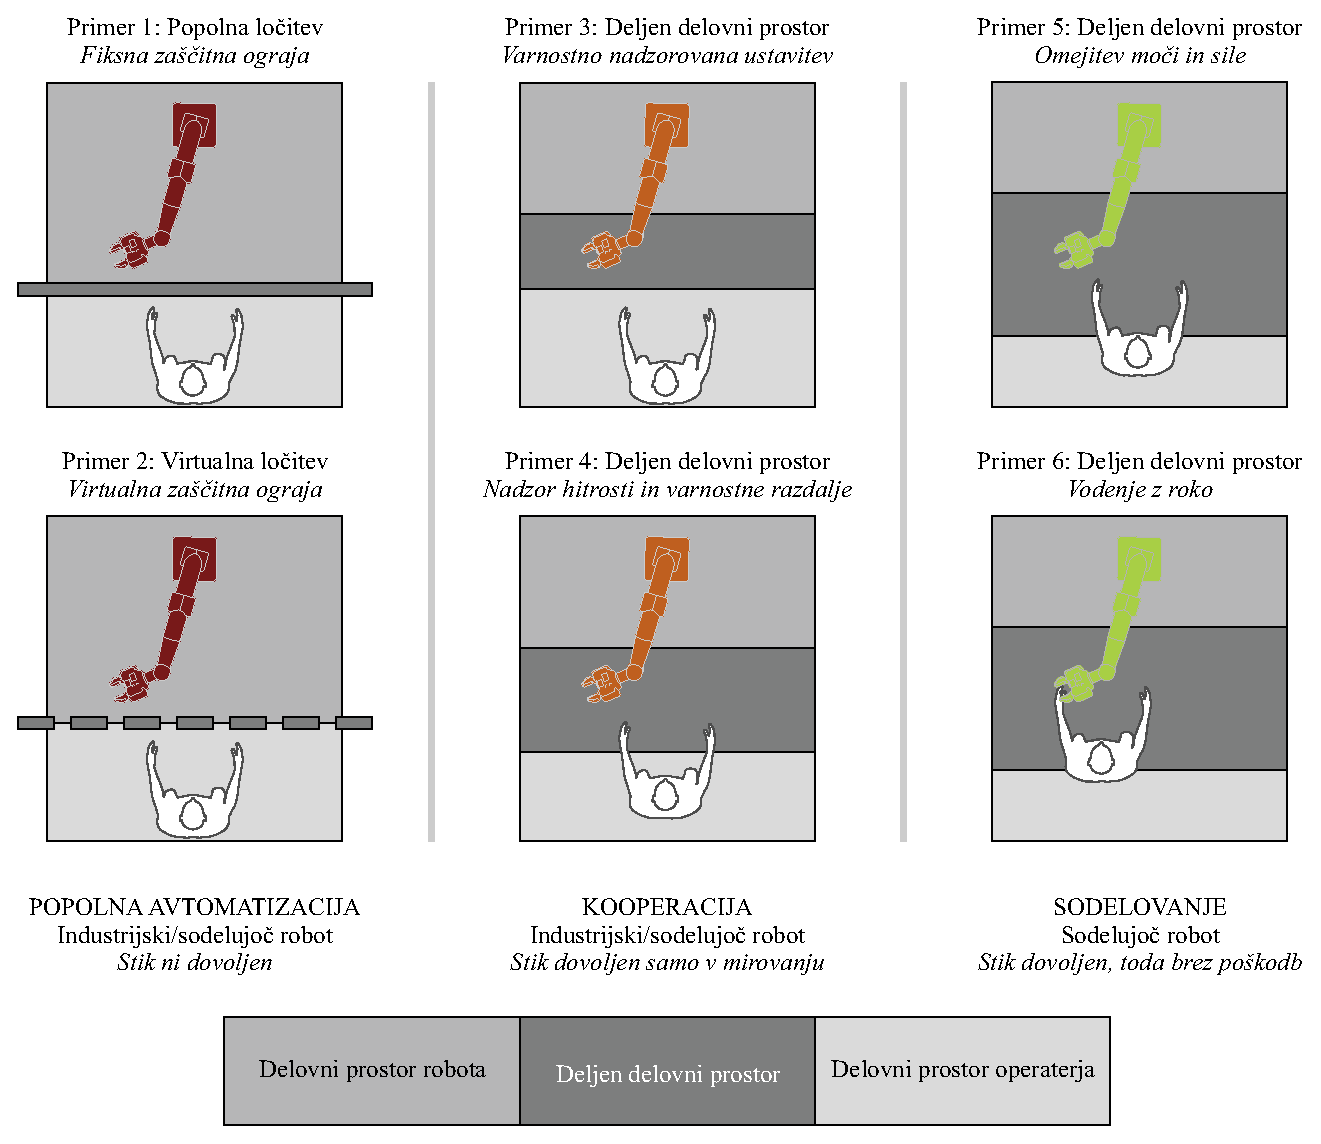
\includegraphics[width=\textwidth]{hc10_sodelovanje.eps}
	\caption{Primeri različnih načinov sodelovanja človeka in robota}
	\label{fig:hc10_sodel}
\end{figure}


Za zagotavljanje varnosti operaterja mora imeti robot implementirano vsaj eno izmed štirih kategorij varnosti:
\begin{itemize}
	\item \textbf{varnostno nadzorovana ustavitev} -- v primeru nevarne situacije se robot ustavi (motorji so prižgani),
	\item \textbf{vodenje z roko}  -- operater lahko ročno vodi robota, enostavnejše programiranje in izvajanje aplikacij,
	\item \textbf{nadzor hitrosti in varnostne razdalje} -- hitrost robota se prilagaja glede na oddaljenost človeka od robota (različne cone hitrosti, bližje kot je operater robotu, manjša je hitrost), potrebni dodatni senzorji (laserski skenerji, svetlobne zavese, ...)
	\item \textbf{omejitev moči in sile} -- robot deluje z ustrezno močjo, da v primeru nehotenega trka z operaterjem ne pride do poškodbe, ISO/TS 15066:2016 podaja ustrezne sile/pritiske za posamezna področja človeškega telesa, kompromis med hitrostjo in nosilnostjo robota.
\end{itemize}


\section{Struktura sistema}

Robotski sistem sestavlja sodelujoči robot Yaskawa Motoman HC10DT s krmilnikom YRC1000, robotsko prijemalo OnRobot RG2 ter laserski skener SICK TIM310-1130000. Celotna konfiguracija je predstavljena na sliki \ref{fig:hc10_sistem}.

\begin{figure}[!hbt]
	\centering
	\includegraphics[width=0.9\textwidth]{hc10_sistem.eps}
	\caption{Robotski sistem}
	\label{fig:hc10_sistem}
\end{figure}

\subsection{Motoman HC10DT}

Robot je predstavnik sodelujočih robotov, ki so narejeni za varno delo skupaj s človekom brez dodatnih varnostnih elementov (varnostnih ograj, svetlobnih zaves ...), seveda v skladu z analizo tveganja. Robotska roka je antropomorfne oblike s 6 prostostnimi stopnjami. Posamezni sklep robota je opremljen s senzorjem navora, ki na nivoju sklepa meri interakcijo robota z okolico. Robota se lahko premika z roko, za shranjevanje ukazov pa se lahko uporablja vmesnik na vrhu robota, kar omogoča prihranek časa pri programiranju robota.

Osnovni podatki robotske roke so podani v tabeli \ref{tab:hc10}.

\begin{table}
	\centering
	\caption{Specifikacije robota Yaskawa Motoman HC10DT} \label{tab:hc10}
	\begin{tabular}{|lr|c|}
		\hline   Tip &  & HC10DT \\
		\hline Doseg & & $1,2$ m \\
		\hline Nosilnost  & & $9$ kg \\
		\hline Hitrost vrha& & $1$ m/s \\
		\hline Hitrost vrha (varen način)& & $0,25$ m/s \\
		\hline Ponovljivost pozicioniranja& & $\pm 0.1$ mm \\
		\hline Maksimalna hitrost
		& Os 1 & $130$ $^\circ/s$ \\
		& Os 2 & $130$ $^\circ/s$ \\
		& Os 3 & $180$ $^\circ/s$ \\
		& Os 4 & $180$ $^\circ/s$ \\
		& Os 5 & $250$ $^\circ/s$ \\
		& Os 6 & $250$ $^\circ/s$ \\
		\hline Delovni prostor
		& Os 1 & $\pm180^\circ$\\
		& Os 2 & $\pm180^\circ$\\
		& Os 3 & $-5^\circ/+355^\circ$\\
		& Os 4 & $\pm180^\circ$\\
		& Os 5 & $\pm180^\circ$\\
		& Os 6 & $\pm180^\circ$\\
		\hline   Teža &  & $48$ kg \\
		\hline
	\end{tabular}
\end{table}

Robot lahko deluje v dveh načinih. Prvi je kot klasični industrijski manipulator, kjer je maksimalna hitrost vrha deklarirana na 1000~mm/s. V tem načinu je potrebno robota ločiti od delavcev z varnostnimi elementi (ograje, svetlovne zavese). Drugi način pa je kot sodelujoči robot. V tem načinu je hitrost vrha omejena na 250~mm/s. Pri tej hitrosti in deklarirani nosilnosti robot v primeru trka s človekom ne povzroči poškodbe (glede na specifikacije ISO/TS 15066:2016).

Robota se programira z uporabo ročne učne enote (slika \ref{fig:hc10_pendant}). Ta omogoča premikanje robota, upravljanje s prijemali, pisanje, popravljanje in poganjanje programov ter podobno.

\begin{figure}[!hbt]
	\centering
	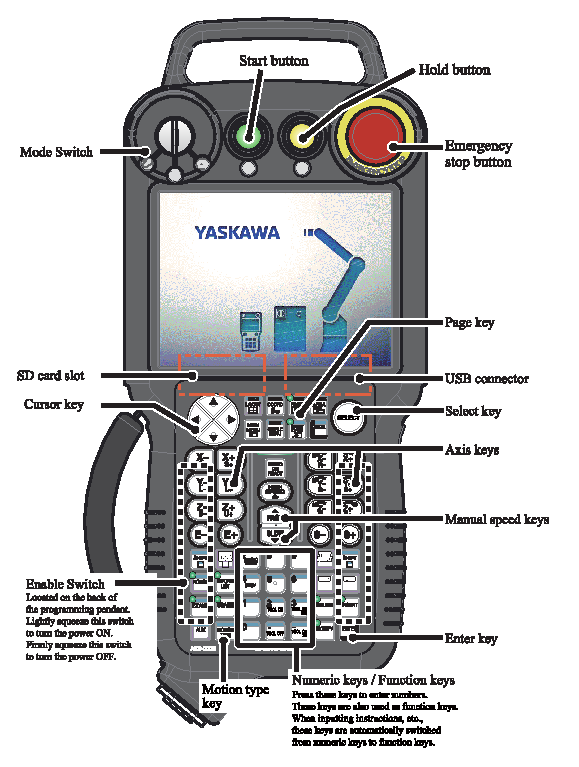
\includegraphics[width=0.9\textwidth]{hc10_pendant.eps}
	\caption{Ročna učna enota}
	\label{fig:hc10_pendant}
\end{figure}

Robot HC10DT je opremljen z integriranim varnostnim krmilnikom FSU (Functional Safety Unit), ki omogoča različne varnostne funkcije. S FSU se lahko nastavi dovoljena območja gibanja posameznega sklepa, maksimalne dovoljene hitrosti za posamezni sklep ter za vrh robota, ter se definira različna območja delovanja (območje, ki ga robot ne sme zapustiti, območje, v katerega robot ne sme vstopiti, ravnine, ki omejujejo gibanje robota).




\subsection{Prijemalo OnRobot RG2}

Prijemalo OnRobot RG2 spada v kategorijo sodelujočih prijemal. Prijemalo omogoča pozicijsko vodenje in vodenje po sili, obenem pa ima integrirano detekcijo stanja prijemanja (objekt prijet/spuščen, prijemanje, širina prijetega objekta). Konfiguracija prstov omogoča tako zunanje kot tudi notranje prijemanje objektov. Specifikacije prijemala so podane v tabeli \ref{tab:RG2}, dimenzije pa so predstavljene na sliki \ref{fig:hc10_onrobot}.

\begin{table}
	\centering
	\caption{Specifikacije prijemala OnRobot RG2}
	\label{tab:RG2}
	\begin{tabular}{|l|c|}
		\hline Tip                  & OnRobot RG2 \\
		\hline Premik prstov        & $0-110$ mm \\
		\hline Ponovljivost prstov   & $\pm 0,1$ mm \\
		\hline Sila prijemanja      & $3-40$ N \\
		\hline Ponovljivost sile    & $\pm 1$ N \\
		\hline Teža                 & $0,65$ kg \\
		\hline
	\end{tabular}
\end{table}


\begin{figure}[!hbt]
	\centering
	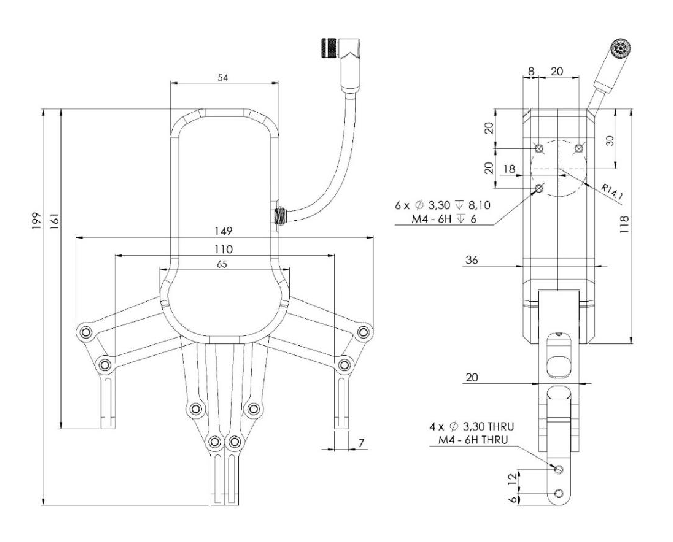
\includegraphics[width=0.9\textwidth]{hc10_onrobot.eps}
	\caption{Dimenzije prijemala OnRobot RG2}
	\label{fig:hc10_onrobot}
\end{figure}


\subsection{Laserski skener SICK TIM310}

Laserski skener SICK TIM310 detektira objekte v različnih področjih glede na odboj laserskega žarka. Doseg skeniranje je do 4~m. Senzor podpira nastavitev treh delno prekrivajočih področij enake oblike vendar različnih velikosti (glej sliko \ref{fig:hc10_sick}). Oblike področij so  v naprej definirane ali pa jih uporabnik nastavi sam. Senzor sporoča v katerem polju se nahaja objekt preko digitalnih linij (vsako področje ima ločeno linijo), zato je z robotskim krmilnikom (FSU) povezan preko digitalnih vhodov.

\begin{figure}[!hbt]
	\centering
	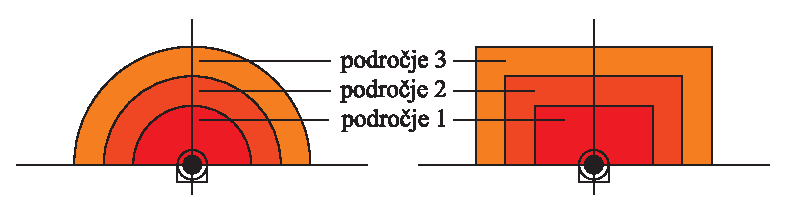
\includegraphics[width=0.9\textwidth]{hc10_podrocja.eps}
	\caption{Primera polkrožnega in pravokotnega področja zaznavanja senzorja}
	\label{fig:hc10_sick}
\end{figure}

Za nastavljanje področij in parametrov senzorja se uporablja program SOPAS. Ta omogoča nastavljanje oblike in velikosti področij, odzivni čas zaznave posameznega področja, velikost objektov, ki jih zanemari, in čas signaliziranja o detektiranem objektu.

\section{Ustvarjanje celice v simulacijskem okolju MotoSimEG-VRC} \label{sim0}

Preko AnyDesk programa se povežite na laboratorijski računalnik, ki je namenjen za vajo. Koda računalnika je \verb|296 827 929|, geslo je \verb|student_3krat4|.

MotoSim EG-VRC je simulacijsko okolje za simulacijo in razvoj robotske celice. Na začetku je potrebno ustvariti nov projekt oziroma celico. Kliknite na okroglo ikono z modrim robotom, ki vam odpre meni za ustvarjanje novih projektov, izberite New/New. Shranite projekt (recimo \verb|HC_10_vaja.vcl|). Odpre se vam okno s 3D pogledom na virtualno celico (zeleno karirasta ravnina), ki še ne vsebuje nobenega robota. V celico je potrebno vstaviti HC10 robota. V zavihku Controller izberemo ikono New, nato pa izberemo opcijo New VRC Controller (no file). Odpre se okno New Controller in v Controller Type izberemo YRC1000 krmilnik. Odpre se novo okno z različnimi možnostimi za robote, ki jih podpira izbrani krmilnik. V Control Group pod možnostjo R1 izberemo robota 1-06VXHC10-A0*(HC10), pod Application pa možnost General. Glej sliko \ref{fig:VRC_01}. Izbiro potrdimo s klikom na gumb Standard Setting Execute, ter OK v naslednjem oknu, ki se odpre.

\begin{figure}[hbt]
	\centering
	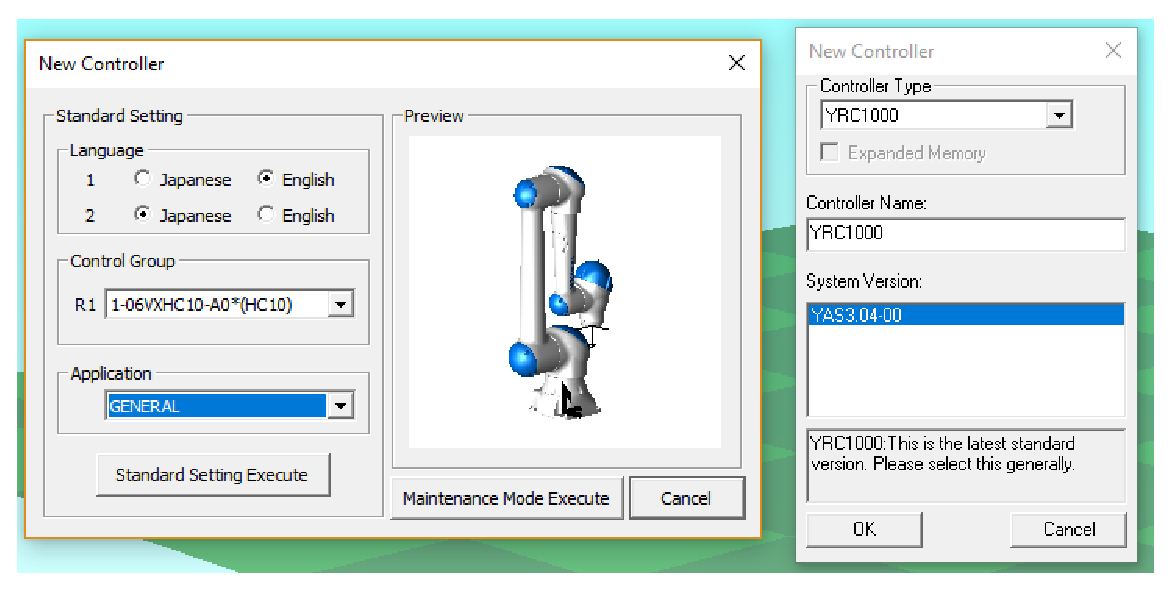
\includegraphics[width=0.5\textwidth]{VRC_01.eps}
	\caption{Izbira ustreznega krmilnika in robota.}
	\label{fig:VRC_01}
\end{figure}

Po potrditvi se bo v prikazu navidezne celice prikazal HC10 robot. Naslednji korak je, da vključimo FSU enoto (Functional Safety Unit). Izberemo ikono Maintenance Mode v polju Boot (meni Controller). Prikazal se bo zaslon navidezne učne enote, v katerm izberemo tipko SYSTEM in nato SETUP. Glej sliko \ref{fig:VRC_02}. Premaknite se do opcije OPTION FUNCTION in jo izberite s tipko SPACE. Kliknite v zaslon navidezne učne enote, pomikate se lahko bodisi z vašo tipkovnico, ki jo imate priključeno na računalnik (pomikate se s smernimi puščicami, izbiro pa potrdite s tipko SPACE) ali pa odprete tipkovnico navidezne učne enote (ikona desno zgoraj na navidezni učni enoti).

\begin{figure}[hbt]
	\centering
	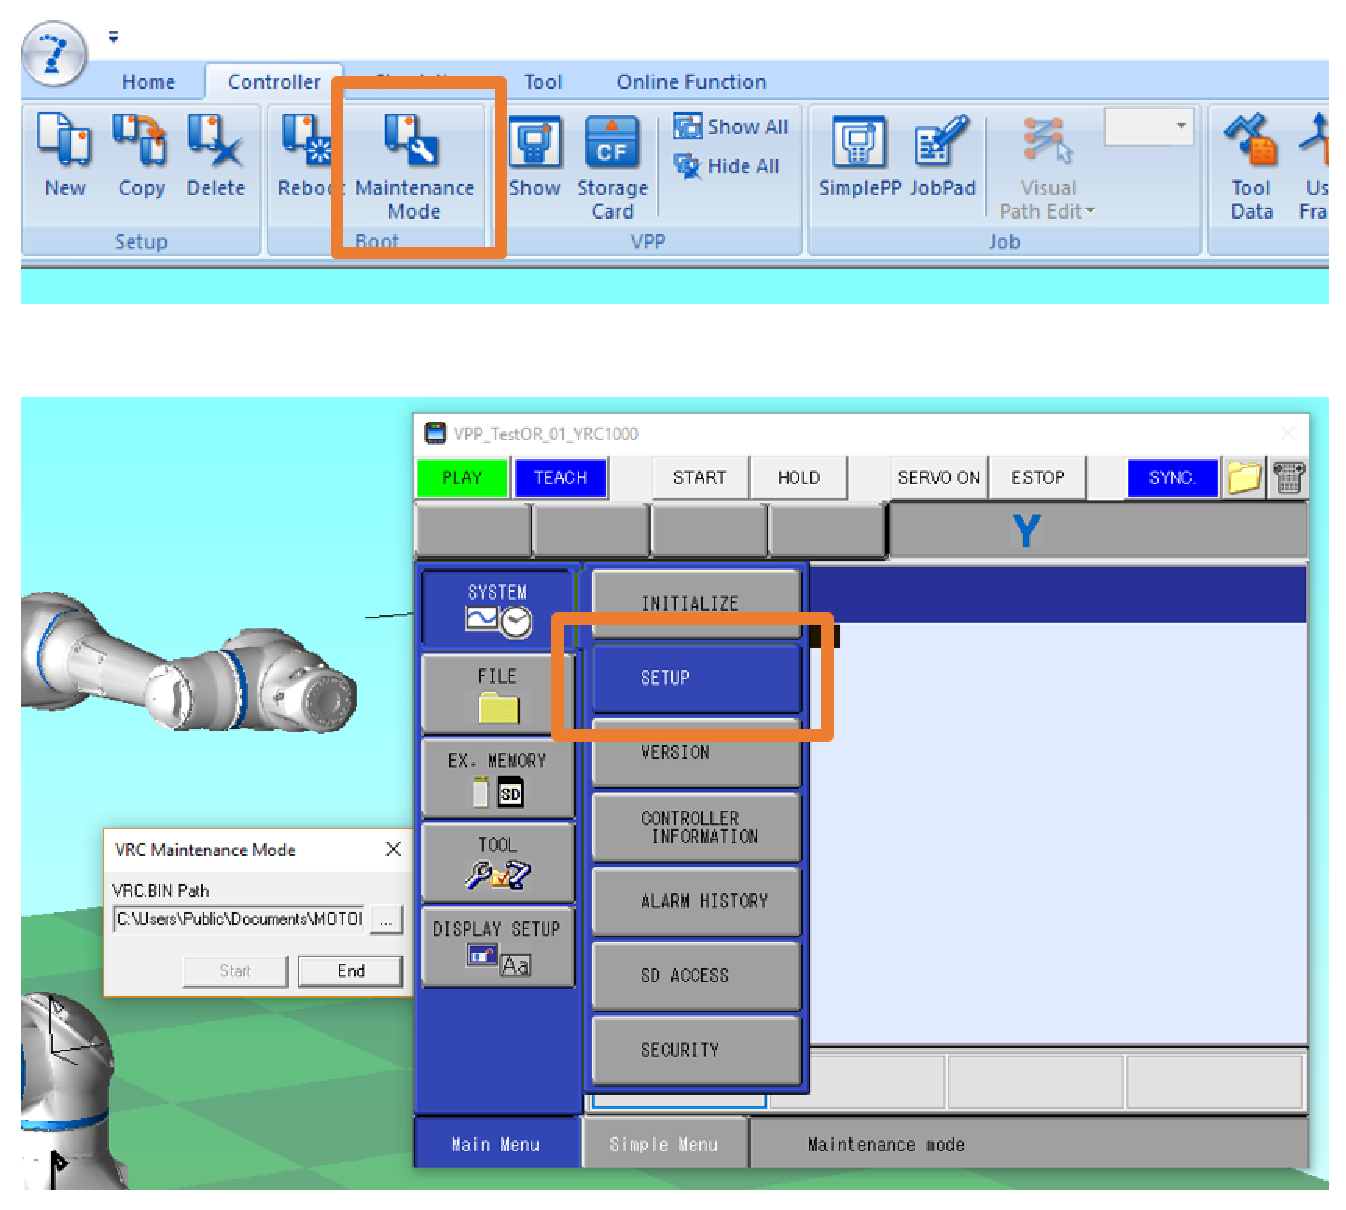
\includegraphics[width=0.5\textwidth]{VRC_02.eps}
	\caption{Maintanence Mode navideznega krmilnika.}
	\label{fig:VRC_02}
\end{figure}

Nato izberemo vrstico 049 Functional safety, pod naslednjim menijem pa pod možnostjo Functional safety izberemo USED (glej sliko \ref{fig:VRC_03}) in, ko se odpre okno Modify, izberemo YeES in še enkrat YES v naslednjem oknu, ki se odpre. Izbiro YES potrdimo z ENTER tipko na tipkovnici. Na koncu navidezno učno enoto zaprete s klikom na gumb Endv oknu VRC Maintanence Mode MotoSim EG-VRC programa.

\begin{figure}[hbt]
	\centering
	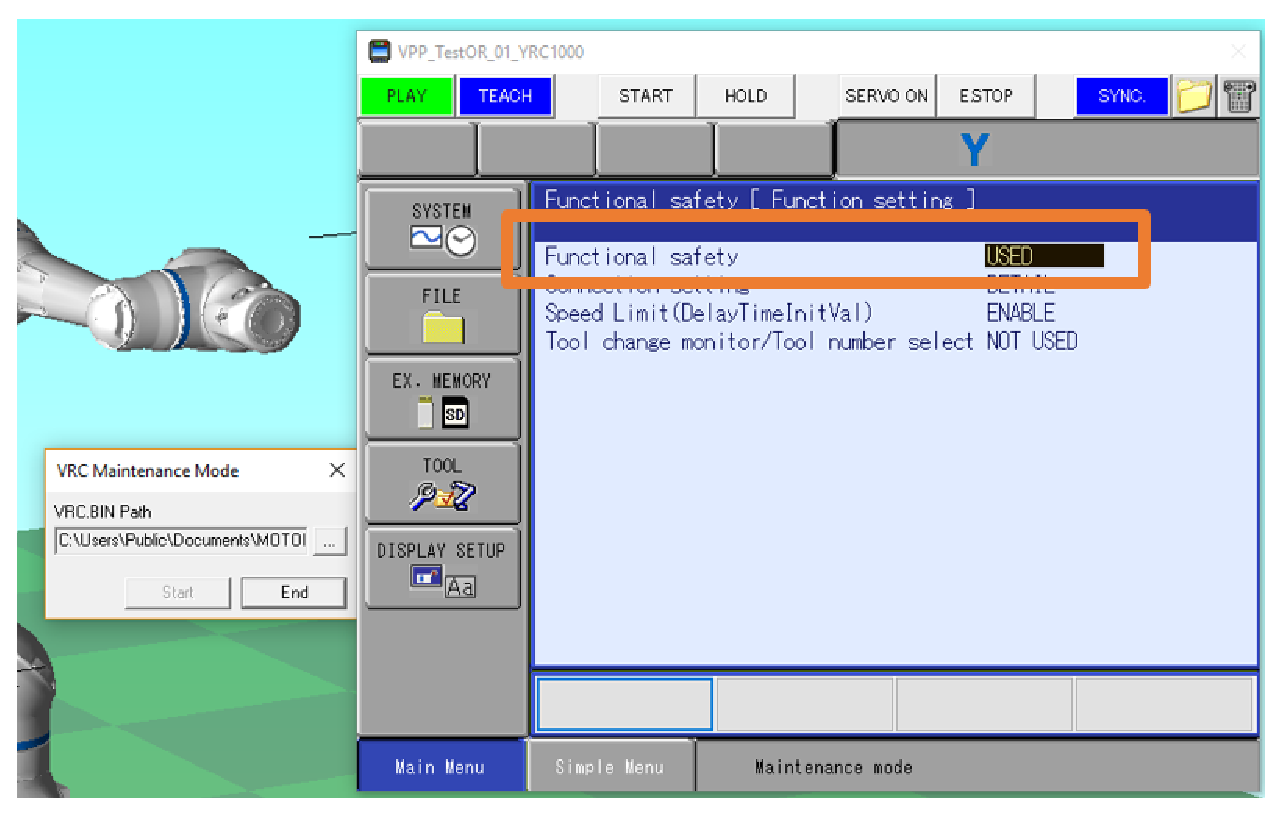
\includegraphics[width=0.5\textwidth]{VRC_03.eps}
	\caption{Vklop FSU enote.}
	\label{fig:VRC_03}
\end{figure}

S tem korakom smo ustvarili osnovno navidezno robotsko celico z ustreznim krmilnikom in robotom, ki je enak dejanskemu krmilniku in robotu v Laboratoriju za robotiko. Robota je sedaj mogoče premikati z navidezno učno enoto kot dejanskega robota na dejanski učni enoti. Navidezno učno enoto v MotoSim vključimo v zavihku Controller in izbiro tipke Show v VPP razdelku. Tipkovnico navidezne učne enote vklopimo z izbiro tipke za VPP tipkovnico. Glej sliko \ref{fig:VRC_04}. Navidezna učna enota je ekvivalent dejanske učne enote prikazane na sliki \ref{fig:hc10_pendant}.

\begin{figure}[hbt]
	\centering
	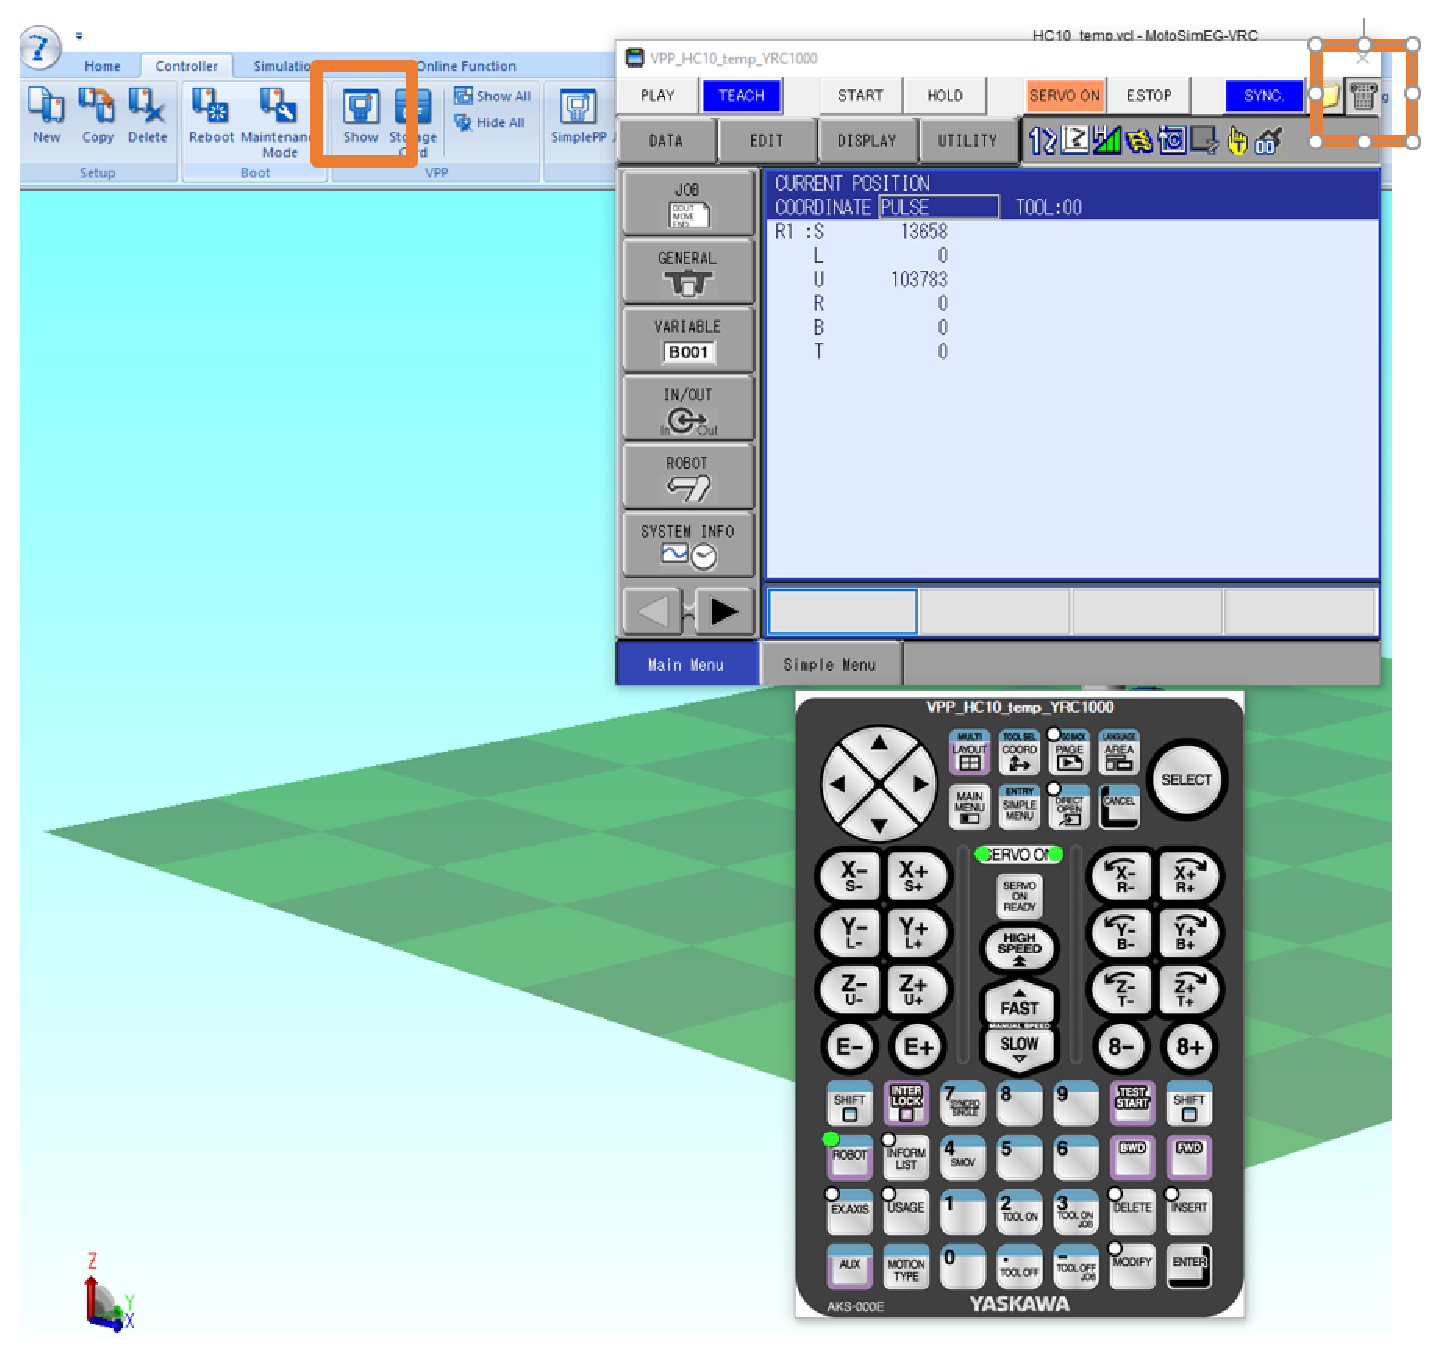
\includegraphics[width=0.7\textwidth]{VRC_04.eps}
	\caption{Navidezna učna enota.}
	\label{fig:VRC_04}
\end{figure}

\clearpage
%\newpage

\section{I. del: Definiranje orodja in objektov}

\subsection{Izvedba v simulaciji} \label{sim1}

\subsection*{Uvoz 3D modela prijemala}

Na robota bomo namestili 3D model prijemala OnRobot RG2, ki je nameščen na dejanskega robota. V zavihku Home izberemo ikono CadTree, ki vklopi okno Cad Tree world okno, ki prikazuje drevo scene navideznega okolja. V Cad drevesu odpremo vse nivoje robota, dokler ne pridemo do zadnjega nivoja YRC1000-R01\_flange. Izberemo  YRC1000-R01\_flange. Izberemo tipko Add, ter v File Name izberemo model orodja \verb|RG2 Gripper 3DModel_Full.stp| (datoteka modela se nahaja na \verb|C:\VAJE\OR\HC_10|). V nadaljevanju potrdimo vsa vprašanja. Orodje se bo pojavilo na mestu pod YRC1000-R01\_flange, če se vam pojavi na katerem od drugih nivojev, ga je potrebno prestaviti na pravo mesto v strukturi drevesa. Glej sliko \ref{fig:VRC_05}.

\begin{figure}[hbt]
	\centering
	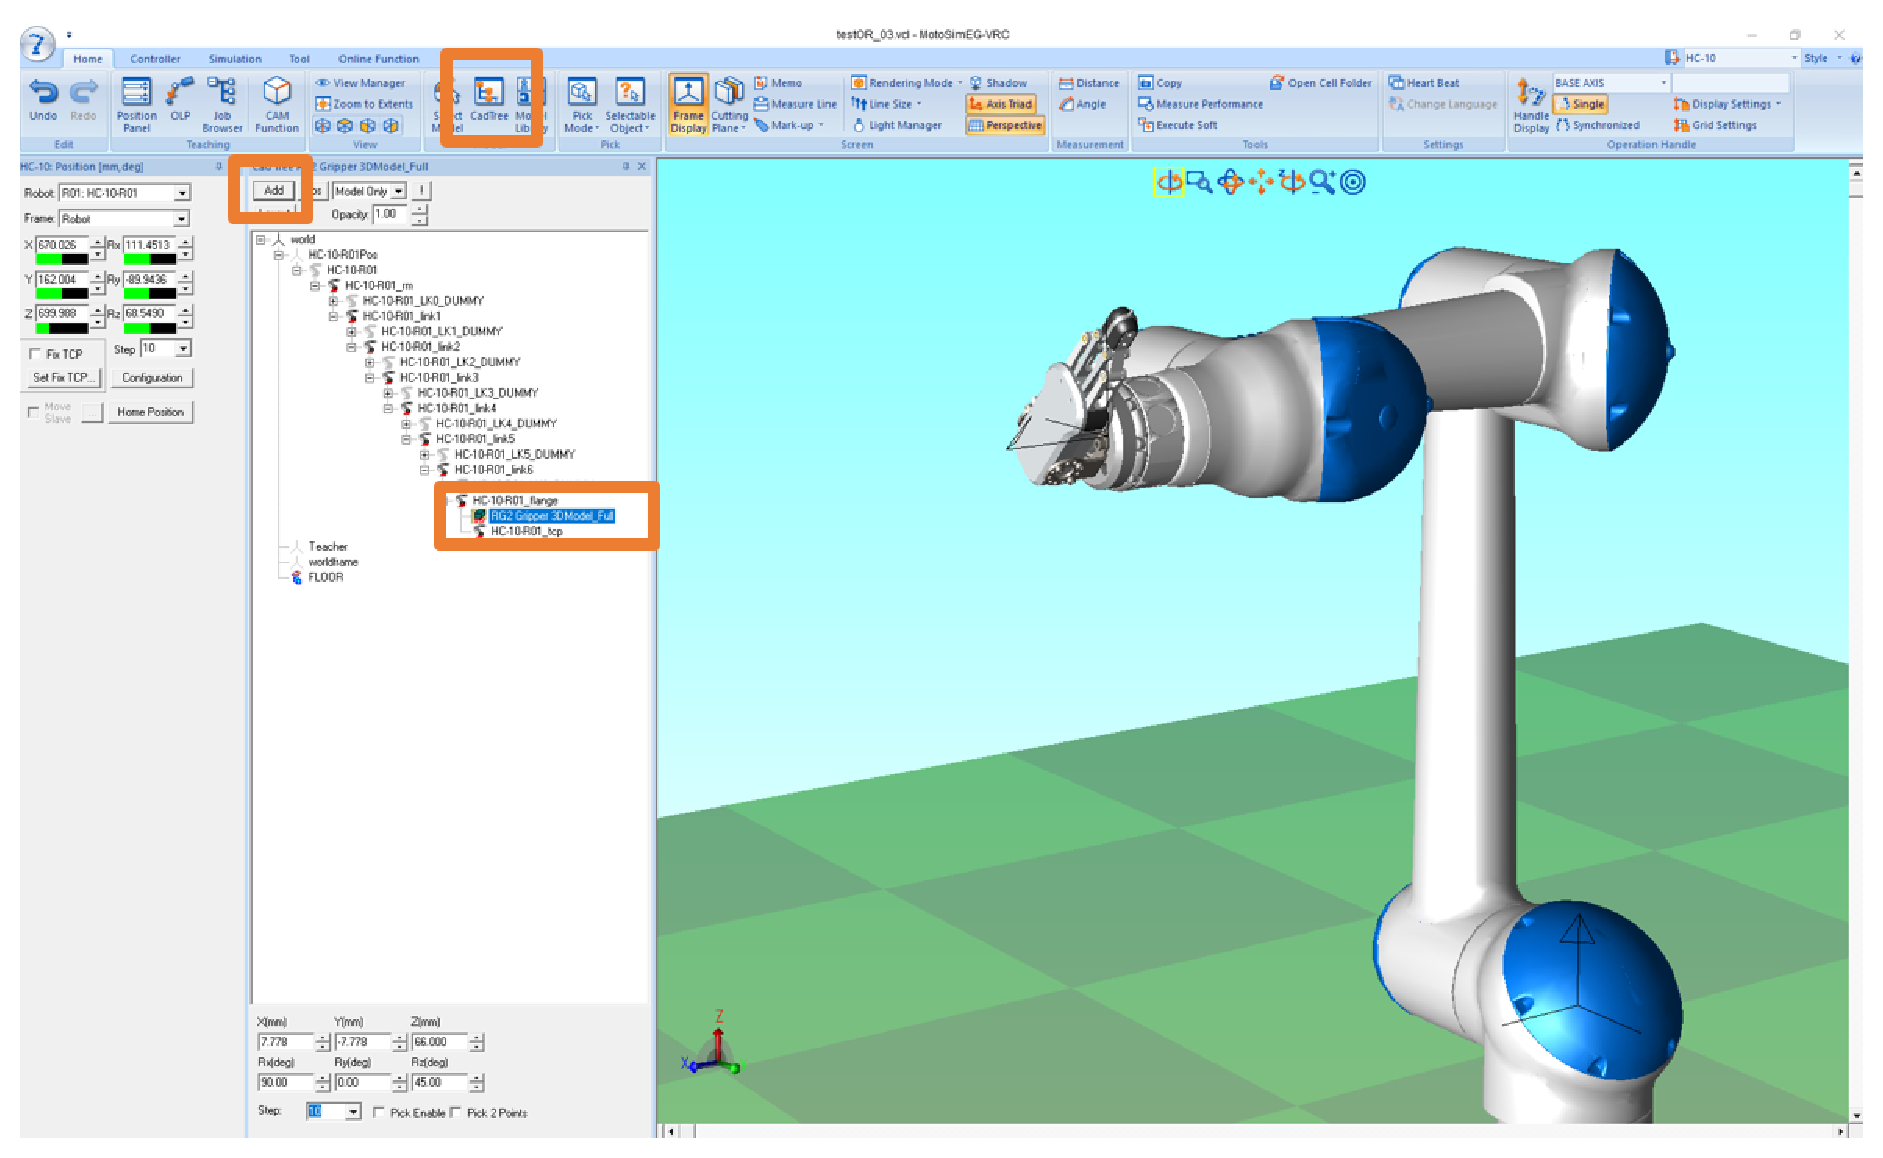
\includegraphics[width=1.0\textwidth]{VRC_05.eps}
	\caption{Vključitev 3D modela prijemala.}
	\label{fig:VRC_05}
\end{figure}

Da je model pravilno postavljen glede na prirobnico robota, je potrebno še vpisati pravilne vrednosti postavitve, ki so zapisane na sliki \ref{fig:VRC_06}.

\begin{figure}[hbt]
	\centering
	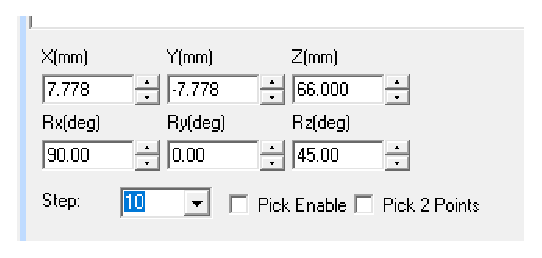
\includegraphics[width=0.4\textwidth]{VRC_06.eps}
	\caption{Pravilne vrednosti postavitve modela orodja na prirobnico robota.}
	\label{fig:VRC_06}
\end{figure}

\subsection*{Kalibracija orodja}

Za kalibracijo orodja je potrebno v zavihku Controller izbrati ikono Tool Data. Odpre se okno za kalibracijo orodja. Najbolj preprosto je opraviti kalibracijo tako, da izberete možnost Pick Enable in kliknete na špico, ki jo ima orodje v prijemalu (glej sliko \ref{fig:VRC_07}).

\begin{figure}[hbt]
	\centering
	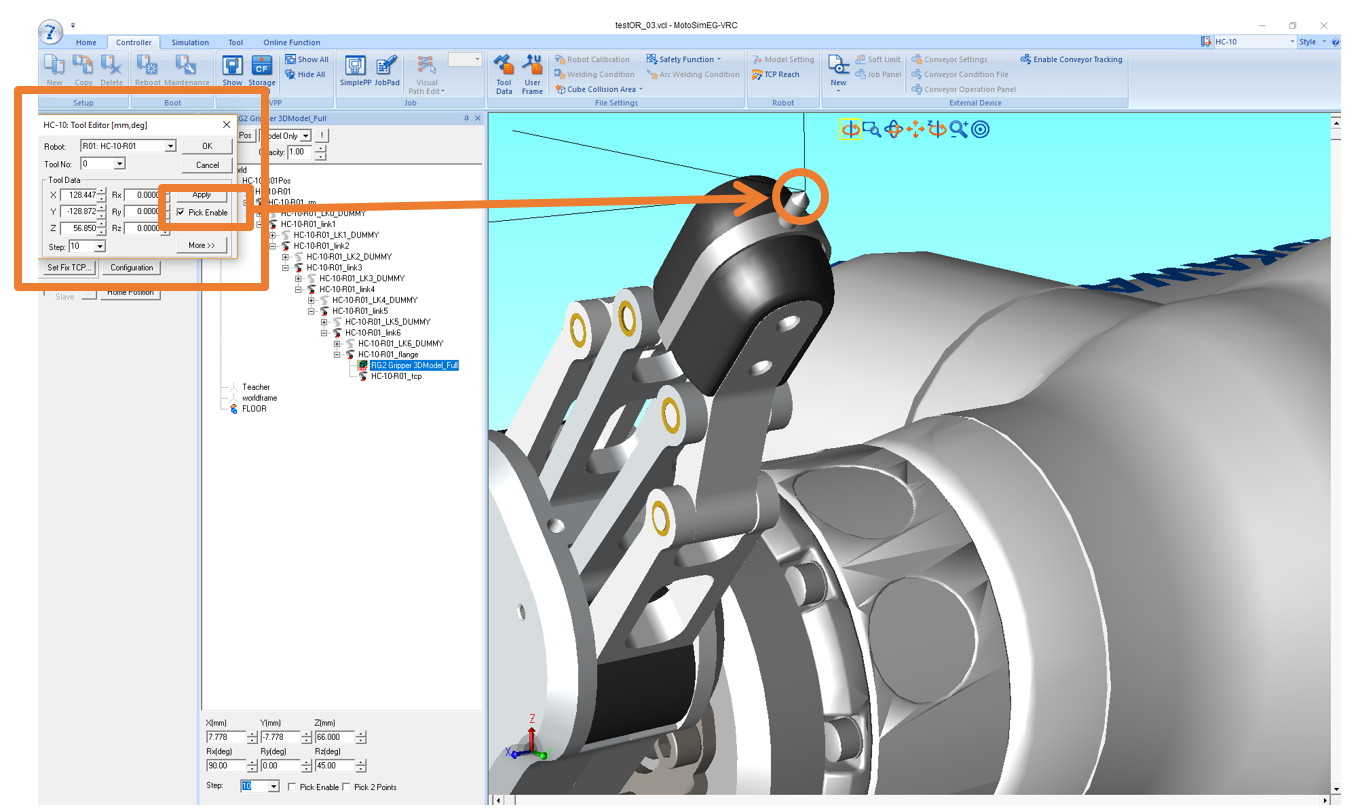
\includegraphics[width=0.9\textwidth]{VRC_07.eps}
	\caption{Prvi korak kalibracije orodja.}
	\label{fig:VRC_07}
\end{figure}

 S tem določimo točko vrha orodja, ne pa tudi orientacije orodja. Prave vrednosti za orientacijo so zapisane na sliki \ref{fig:VRC_08}.
 
\begin{figure}[hbt]
	\centering
	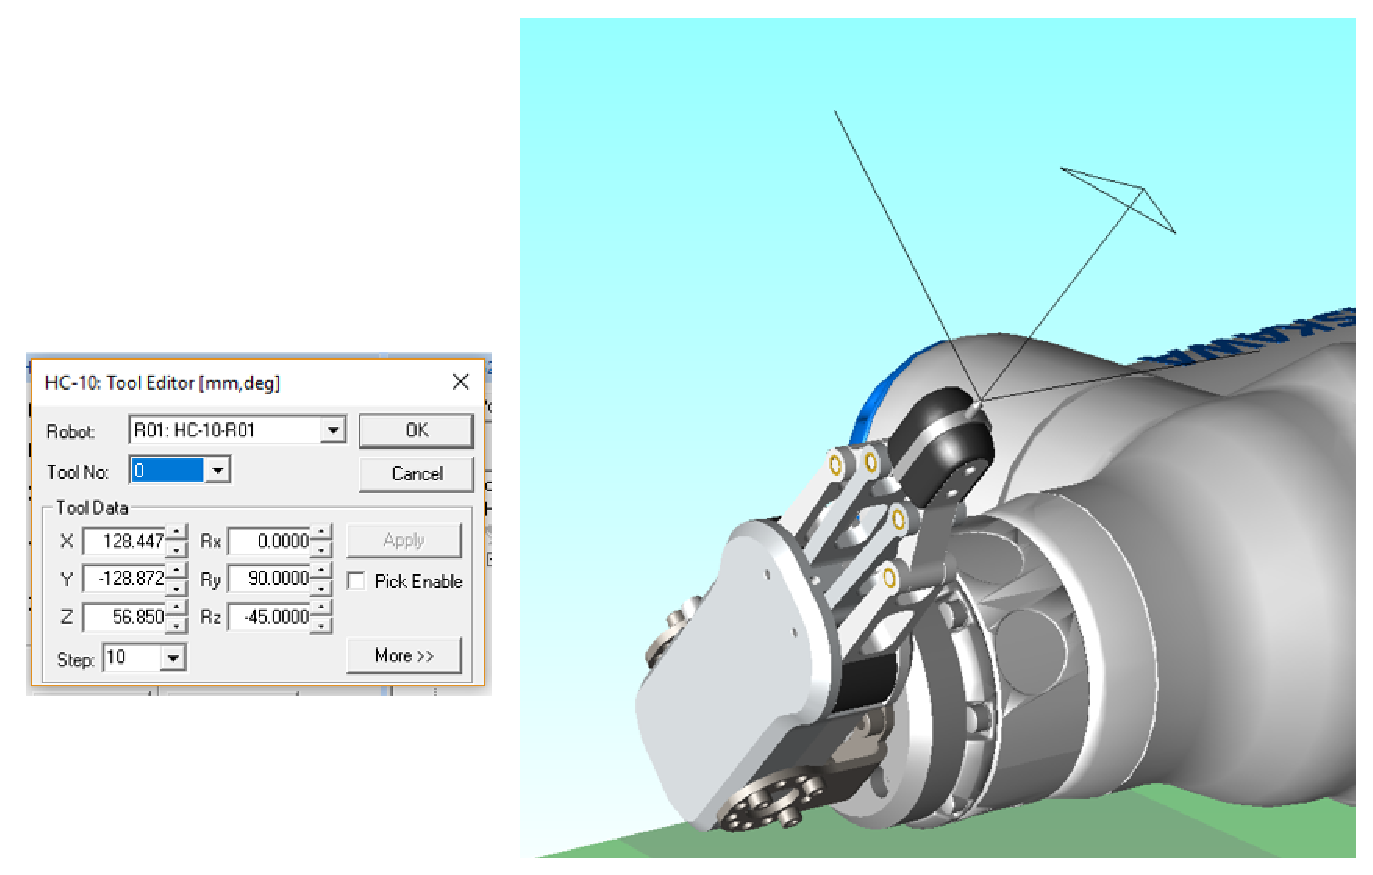
\includegraphics[width=0.8\textwidth]{VRC_08.eps}
	\caption{Določitev orientacije orodja.}
	\label{fig:VRC_08}
\end{figure}

\subsection*{Varnostna ovojnica prijemala}

Po deklaraciji je potrebno orodju določiti še parametre varnostne ovojnice valjev za detekcijo trkov z navideznimi varnostnimi območji. Varnostno ovojnico dodamo z izbiro Tool Interference Model (glej sliko \ref{fig:VRC_09}).

\begin{figure}[hbt]
	\centering
	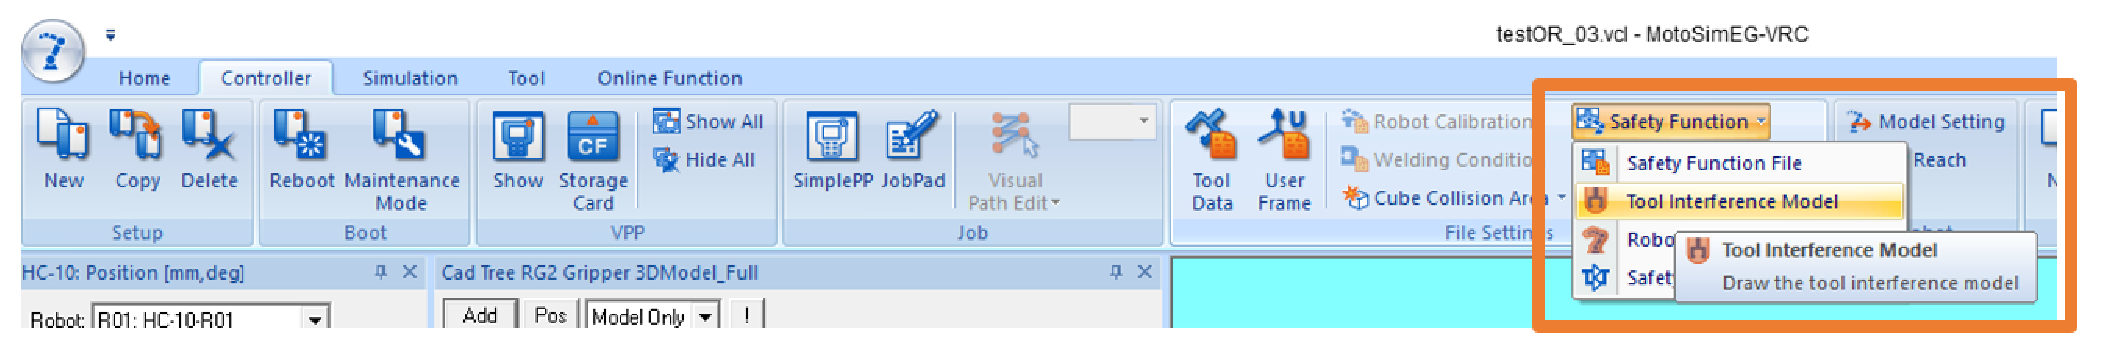
\includegraphics[width=0.9\textwidth]{VRC_09.eps}
	\caption{Meni Tool Interference Model.}
	\label{fig:VRC_09}
\end{figure}

Dodali bomo dva valja okoli orodja (glej sliko \ref{fig:VRC_12}), vrednosti so zapisane na sliki \ref{fig:VRC_10}. Bodite pozorni na to, da pod \verb|Radius (mm)| vpište vrednost $40$ $mm$. V primeru, da boste pozabili vpisati vrednost, vam bo program vrnil napako, saj mora biti pod radij ovojnice vpisana neničelna vrednost. Na koncu se izbere še Add Model.

\begin{figure}[hbt]
	\centering
	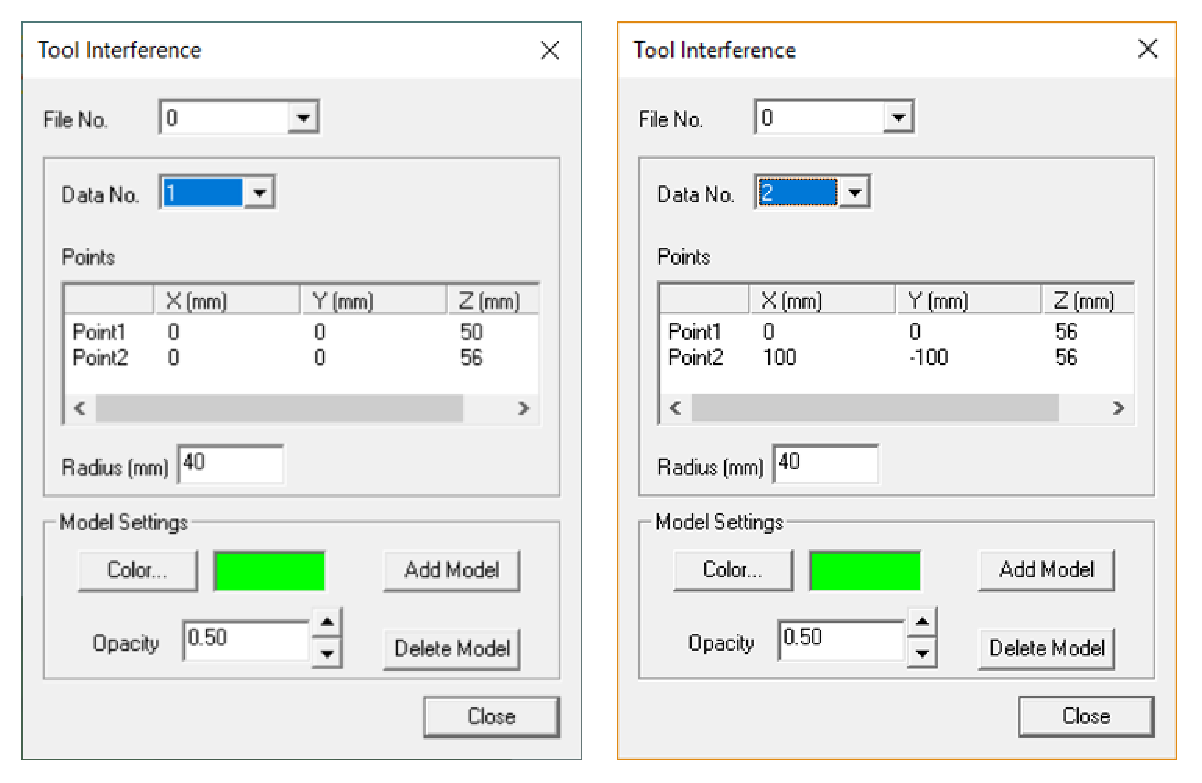
\includegraphics[width=0.7\textwidth]{VRC_20.eps}
	\caption{Vrednosti varnostne ovojnice.}
	\label{fig:VRC_10}
\end{figure}

\subsection*{Definiranje varnostnega območja}

V nadaljevanju preizkusite varnostni mehanizem uporabe navideznih varnostnih območij. Dodajanje varnostnih območij je mogoče v meniju Robot Range Limit. Za prikaz Robot Range Limit, izberete zavihek Controller, polje File Settings, opcija Safety Function/Safety Function File. V oknu Safety Function File Settings-YRC1000 izberete prvi zavihek Robot Range Limit. Izberete ustrezen File No. pod katerega boste zapisali vrednosti za vnos parametrov varnostnega območja. Na koncu še potrdite izbiro prikaza z Add All Model. Če želite izbrisati prikaz varnostnega področja izberite Delete All Model. Izpolnite vrednosti kot so zapisane na sliki \ref{fig:VRC_11}.

\begin{figure}[hbt]
	\centering
	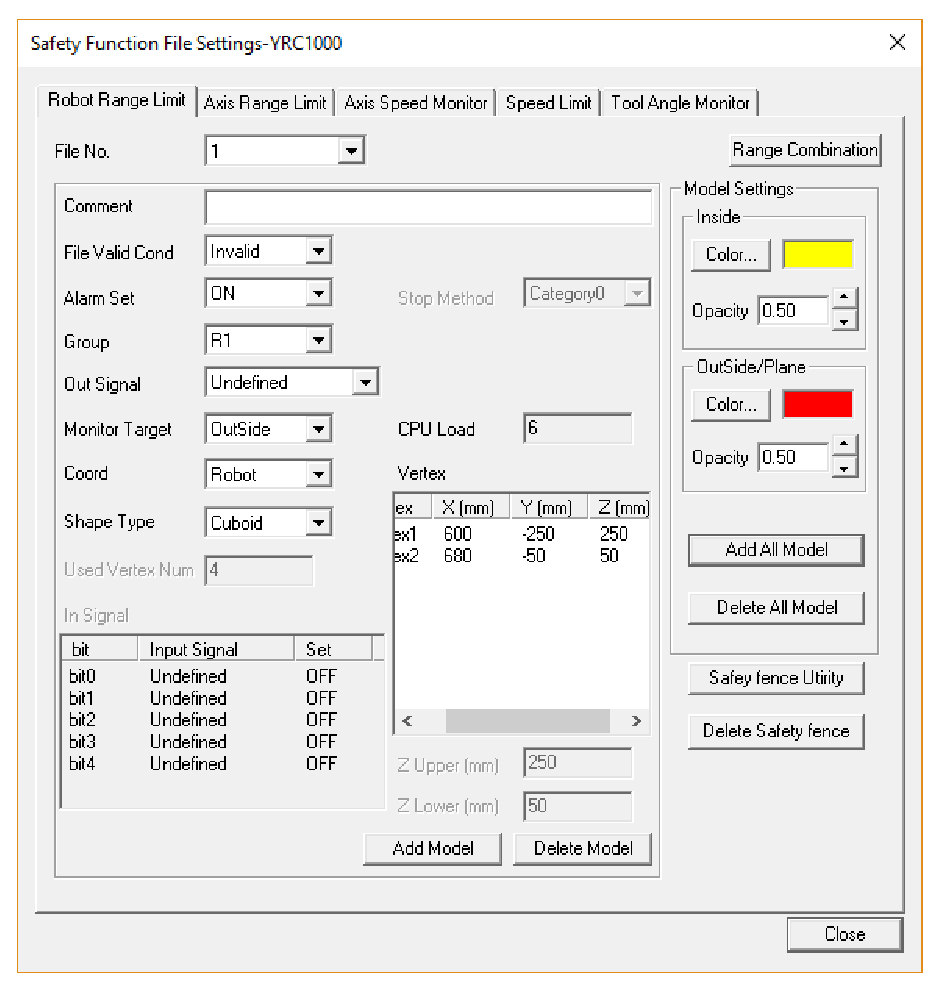
\includegraphics[width=0.7\textwidth]{VRC_11.eps}
	\caption{Vrednosti varnostnega območja.}
	\label{fig:VRC_11}
\end{figure}

Slika \ref{fig:VRC_12} prikazuje postavitev varnostnega območja v delovnem področju robota.

\begin{figure}[hbt]
	\centering
	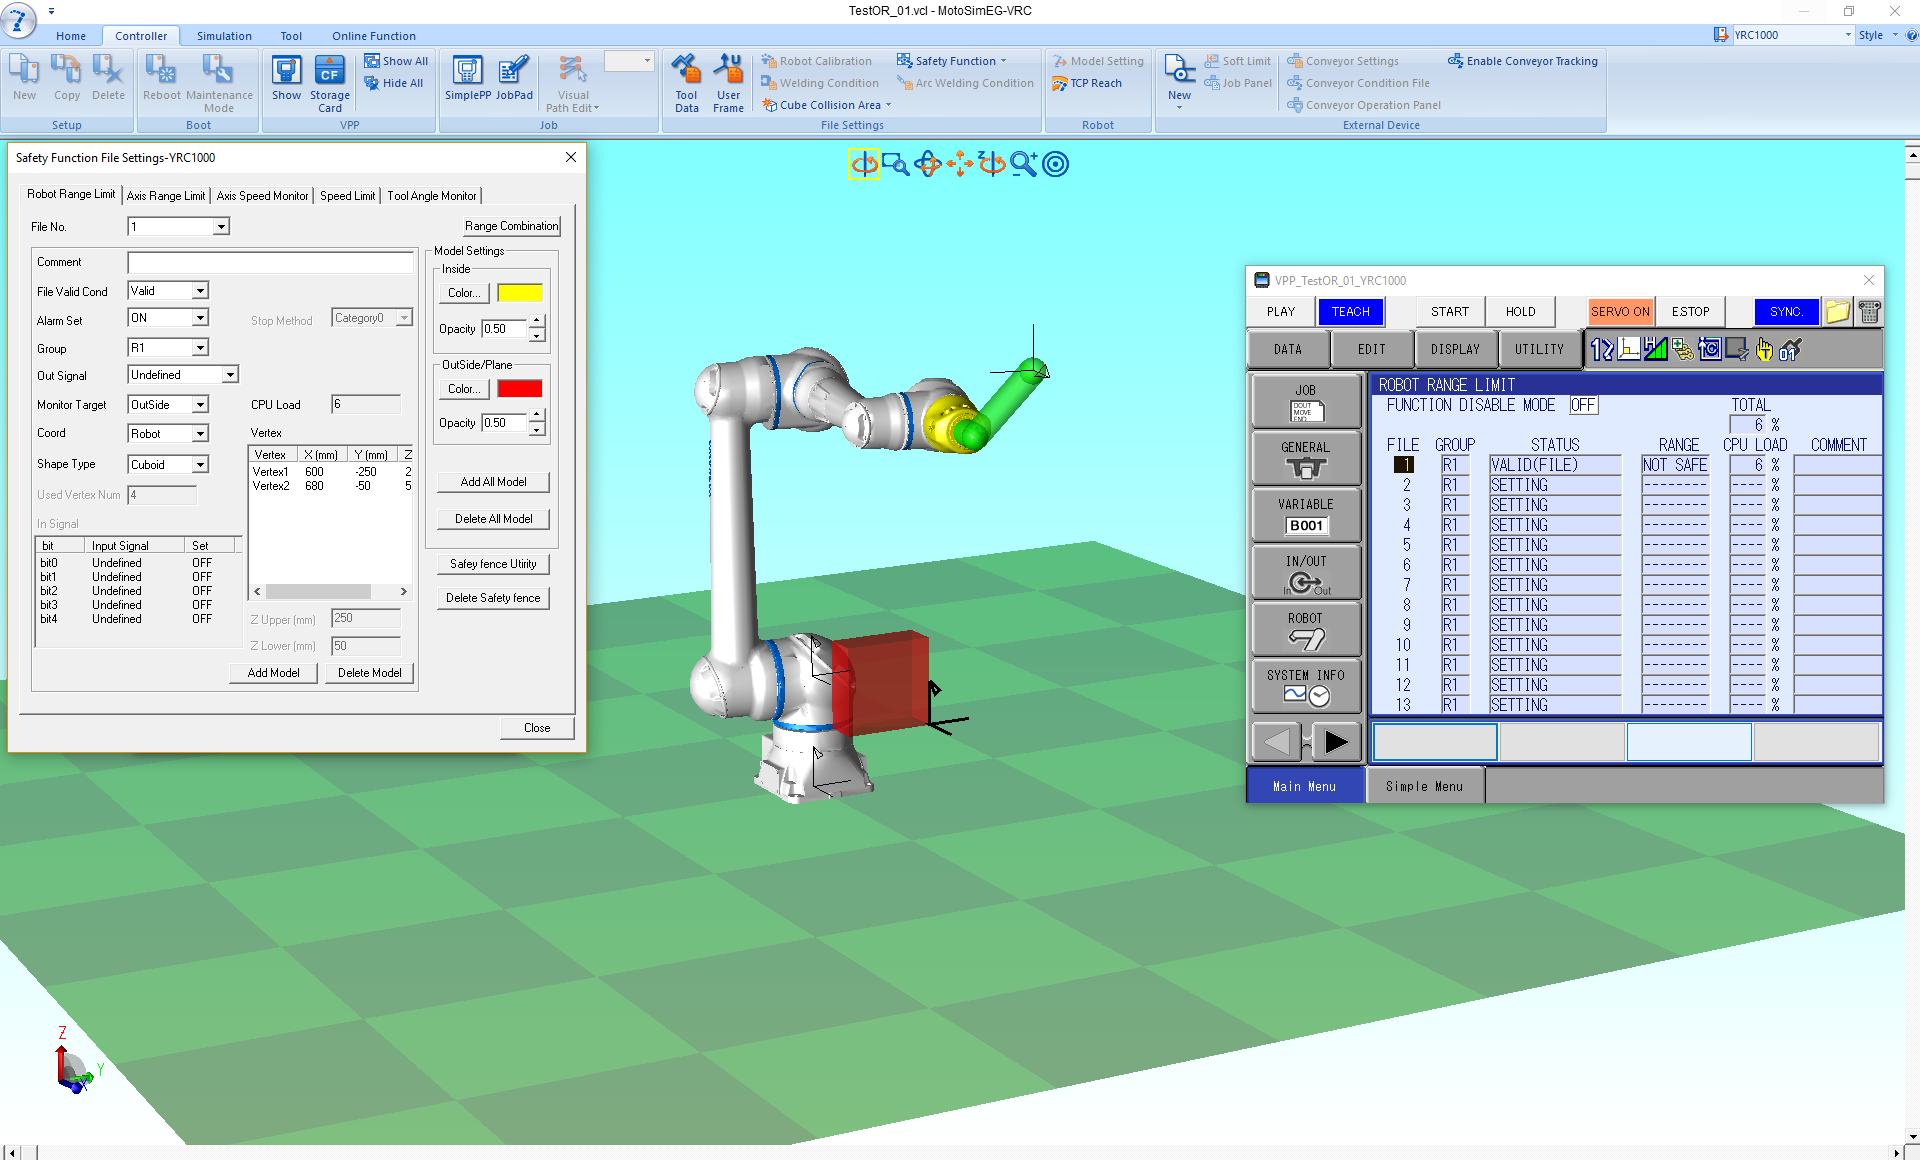
\includegraphics[width=0.7\textwidth]{VRC_12.eps}
	\caption{Postavitev varnostnega območja v delovnem področju robota.}
	\label{fig:VRC_12}
\end{figure}


\subsection*{Test preprečevanja trka med objekti v MotoSim okolju}

V nadaljevanju boste ustvarili program za test preprečevanja trka med objekti. Ustvarjanje programa z navidezno učno enoto je enako kot na dejanski učni enoti. 

V nadaljevanju ustvarite nov robotski program (\textbf{JOB > CREATE NEW JOB}). V polju \textbf{JOB NAME (***)} pritisnete tipko \textbf{SELECT} in odprete okno za definiranje imena programa. Za potrditev imena pritisnete tipko \textbf{ENTER}. Parametre novega programa potrdite s tipko \textbf{EXECUTE}.

Nato postavite robota nad škatlo ter shranite to točko kot linearni gib (ukaz \verb"MOVL V=900"; če je potrebno, ga nastavite s tipko \textbf{MOTION TYPE}). Točko shranite tako, da imate prižgane motorje ter pritisnete tipko \textbf{ENTER}. Robota nato prestavite na eno stran škatle ter to točko ponovno shranite kot \verb"MOVL". Robota prestavite še na drugo stran škatle ter shranite še to točko. Na sliki \ref{fig:VRC_13} je predstavljena shema postavitve točk.

\begin{figure}[hbt]
	\centering
	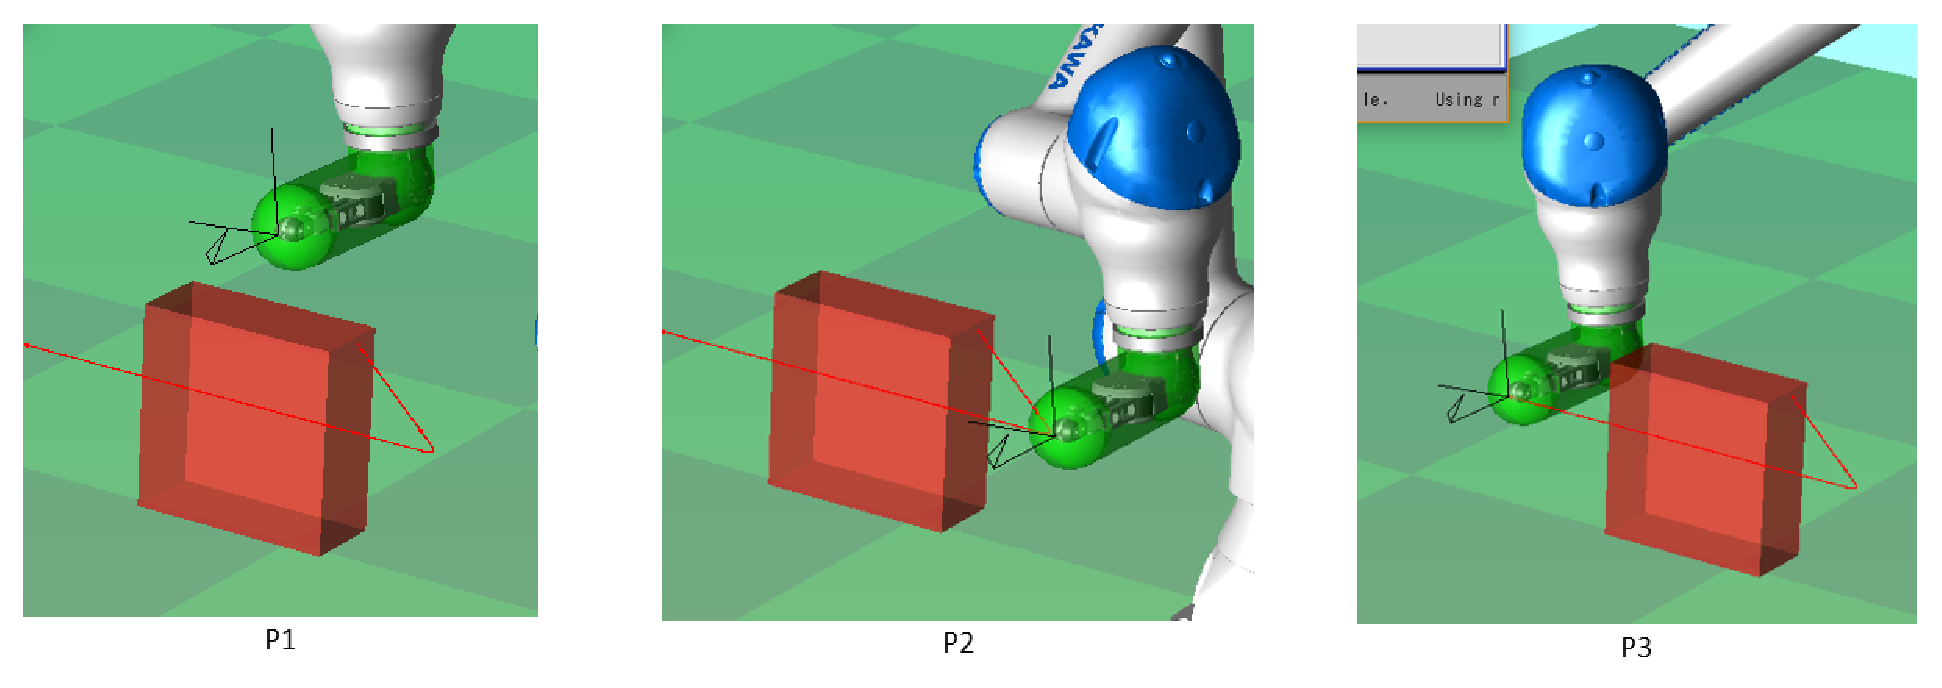
\includegraphics[width=0.7\textwidth]{VRC_13.eps}
	\caption{Postavitev točk za program za testiranje varnostnega območja v delovnem področju robota.}
	\label{fig:VRC_13}
\end{figure}

Program se zažene v navidezni učni enoti. V TEACH načinu se je potrebno premakniti na prvo vrstico (0000 NOP). Preklopiti je potrebno v PLAY način in zagnati program s tipko START. Zaženite prvič program brez vklopljenega varnsotnega področja, drugič pa z vklopljenim varnostnim področjem. Varnostno področje vklopite v meniju Safety Function/Safety Function File/Robot Range Limit. V vrstici File Valid Cond izberite možnost Valid.

\subsection*{Test preprečevanja trka med objekti na dejanskem robotu}

Če želimo testirati trk še na robotu je potrebno prenesti iz MotoSim okolja program in ustrezne konfiguracijske datoteke z navideznega krmilnika na dejanski krmilnik. Na krmilnik robota je potrebno prenesti sam program (JOB), ter definicije orodja in varnostnih področij:
\begin{itemize}
\item Datoteka s končnico JOB vsebuje program.
\item TOOL.CND – vsebuje definicija orodja.
\item TOOLINTF.DAT – vsebuje definicija ovojnice orodja.
\item RBRNGLMT.DAT - vsebuje podatke o prepovedanih območjih znotraj delovnega prostora robota.
\end{itemize}

Najprej je potrebno vpisati nastavitve dejanskega krmilnika kot prikazuje slika . V zavihku Online Function izberete ikono Network. Pojavi se seznam Network Connection. Izberete krmilnik na seznamu (YRC1000) in kliknete na Settings. Pod IP Address vpišete pravilni IP naslov. Za povezovanje MotoSim in dejanskega krmilnika mora biti na dejanski učni enoti izbran Remote mode (glej sliko \ref{fig:VRC_19}).

\begin{figure}[hbt]
	\centering
	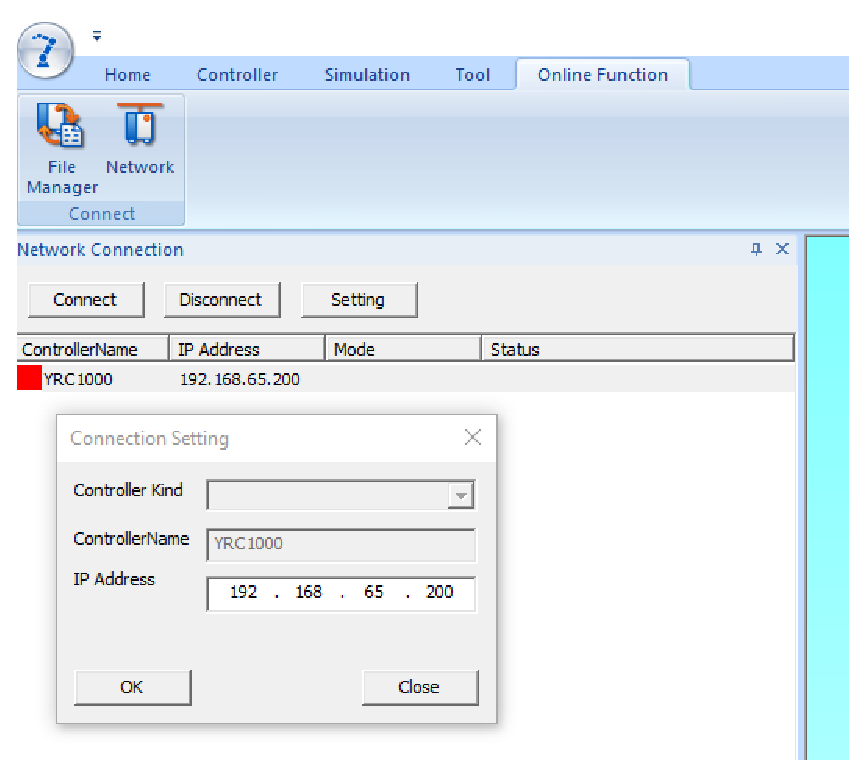
\includegraphics[width=0.5\textwidth]{VRC_18.eps}
	\caption{Mrežne nastavitve za dejanski krmilnik.}
	\label{fig:VRC_18}
\end{figure}

\begin{figure}[hbt]
	\centering
	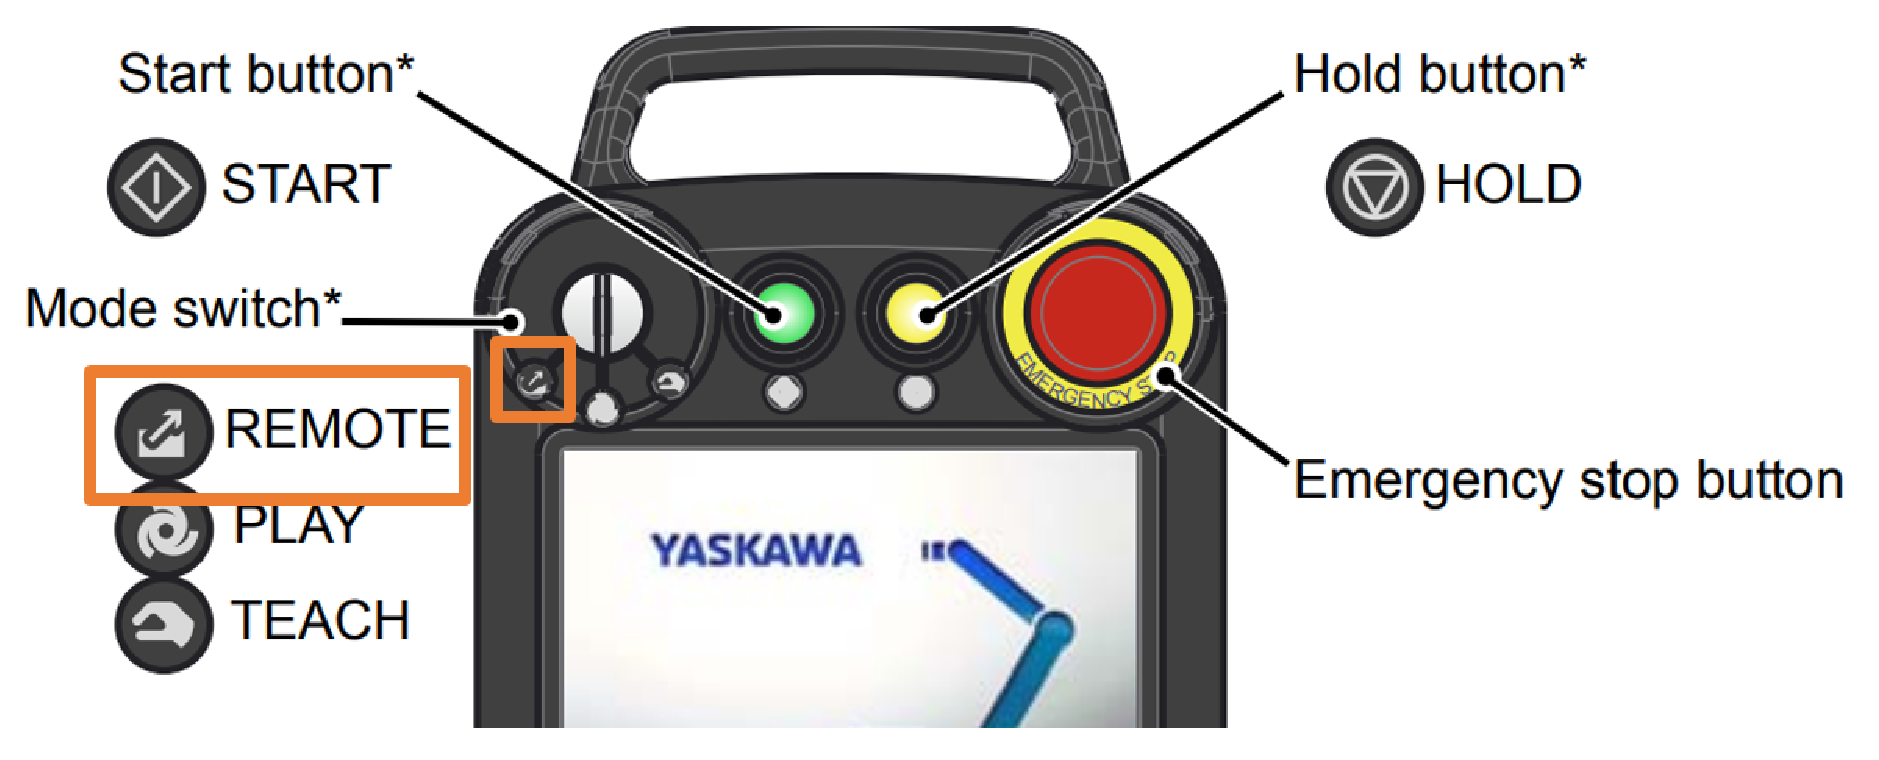
\includegraphics[width=0.5\textwidth]{VRC_19.eps}
	\caption{Remote Mode na dejanski učni enoti.}
	\label{fig:VRC_19}
\end{figure}

\begin{mdframed}[backgroundcolor=red!20, shadow=true,roundcorner=8pt]
	\begin{itemize}
		\item \textbf{Pokličite asistenta, da bo preko USB ključa prenesel datoteke na krmilnik robota in zagnal I. del vaje.}
	\end{itemize}
\end{mdframed}
	
Datoteke je potrebno shraniti na USB ključ, ki se ga vstavi v učno enoto in prenese datoteke na krmilnik. V oknu MotoSimEG-VRC izberete zavihek Online Function. Izberete ikono File Manager. Pod Select VRC izberete YRC1000 (morda bo namesto tega zapisana možnost HC-10). V meniju Category izberete posamezne končnice datotek. V oknu PC izberete ustrezno datoteko ter jo odprete z Edit/File Open. S tem se odpre tekstovni urejevalnik (Notepad) z izbrano datoteko, ki jo lahko potem shranite neposredno na USB ključek s File/Save As (meniju v tekstovnem urejevalniku).


\begin{mdframed}[backgroundcolor=red!20, shadow=true,roundcorner=8pt]
	\begin{itemize}
		\item \textbf{Skupaj z asistentom testirajte izvedbo na robotu.}
	\end{itemize}
\end{mdframed}

\section{II. del: Varnostni odmik robota} \label{poglavje2del_vaje}

Najprej izklopite ovojnico kocke, nato nadaljujte z nalogo. FSU skrbi tudi za implementacijo varnostnega protokola omejtive moči in sile. V tem primeru je kontakt med robotom in uporabnikom dovoljen, saj robot v primeru detektiranja zunanje sile aktivira varnostno nadzorovano ustavitev. Ko uporabnik potrdi, da ni več neželjenega kontakta (restart gumb na petem segmentu), robot nadaljuje z opravljanjem naloge. Zunanja sila je ocenjena na podlagi primerjave izračunanih navorov v sklepih na podlagi trenutne lege robota (in znanih dinamičnih in kinematičnih parametrih robota) ter izmerjenimi navori s sklepnimi senzorji  navora. Razlike med navori se upoštevajo kot sklepni prispevki zunanjih sil, ki delujejo na robota (kontakt).

Robot ima implementiran tudi varnostni odmik v primeru, da je sila interakcije manjša od postavljenega praga za ustavitev robota. V tem primeru ne gre za to, da se robot izogne oviri, ampak se izvede odmik v nasprotni smeri kontakta, da se prepreči poškodbe operaterja. Ko robot zazna, da ni več interakcije z okolico, se vrne v prejšnjo lego in nadaljuje z nalogo. če pa je sila večja od praga, se izvede klasična varnostno nadzorovana ustavitev.

\subsection{Izvedba v simulaciji} \label{sim2}

Izvedba na dejanskem robotu in v MotoSim je podobna. V MotoSim okolju vse korake, ki so opisani v naslednjem delu izvedete s pomočjo navidezne učne enote. Preden začnete pisati program odstranimo prikaz za prepovedano območje: zavihek Controller, ikona Safety Function/Safety Function File. Odpre se okno Safety Function File Settings. V zavihku Robot Range Limit pod File Valid Cond izberemo Invalid, ter v polju Model Settings izberemo gumb Delete All Model.
Ustvarimo program za drugi del (glej sliko \ref{fig:VRC_14}). Ponovno izberemo virtualno učno enoto z ikono Show programing pendant v zavihku Controller. 

\begin{figure}[hbt]
	\centering
	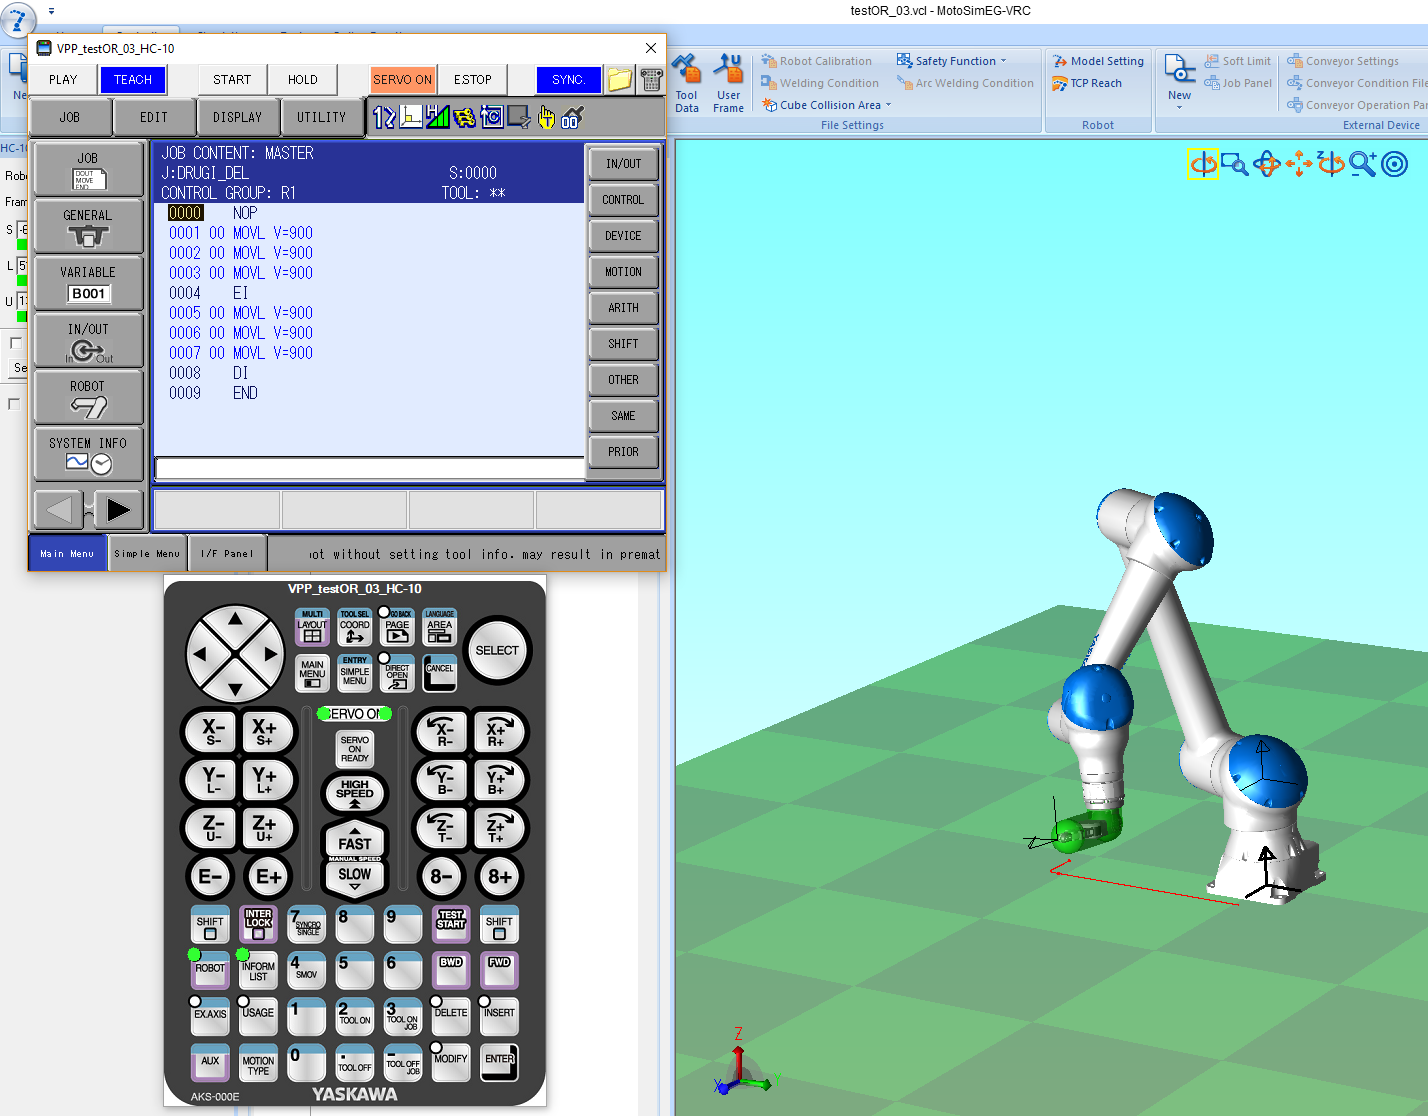
\includegraphics[width=0.7\textwidth]{VRC_14.eps}
	\caption{Priprava programa v okolju MotoSim.}
	\label{fig:VRC_14}
\end{figure}

Ko je program napisan, ga lahko na dejanskega robota prenesete z USB ključem ali pa direktno iz MotoSim okolja na sledeči način. Ko je program ustvarjen, ga je mogoče direktno prenesti na krmilnik. V oknu MotoSimEG-VRC izberete meni Online Function. Izberete ikono File Manager. Pod Select VRC izberete HC-10. V meniju Category izberete JOB. Izberete JOB datoteko za drugi del in jo prenesete na krmilnik s File/Copy.

\begin{figure}[hbt]
	\centering
	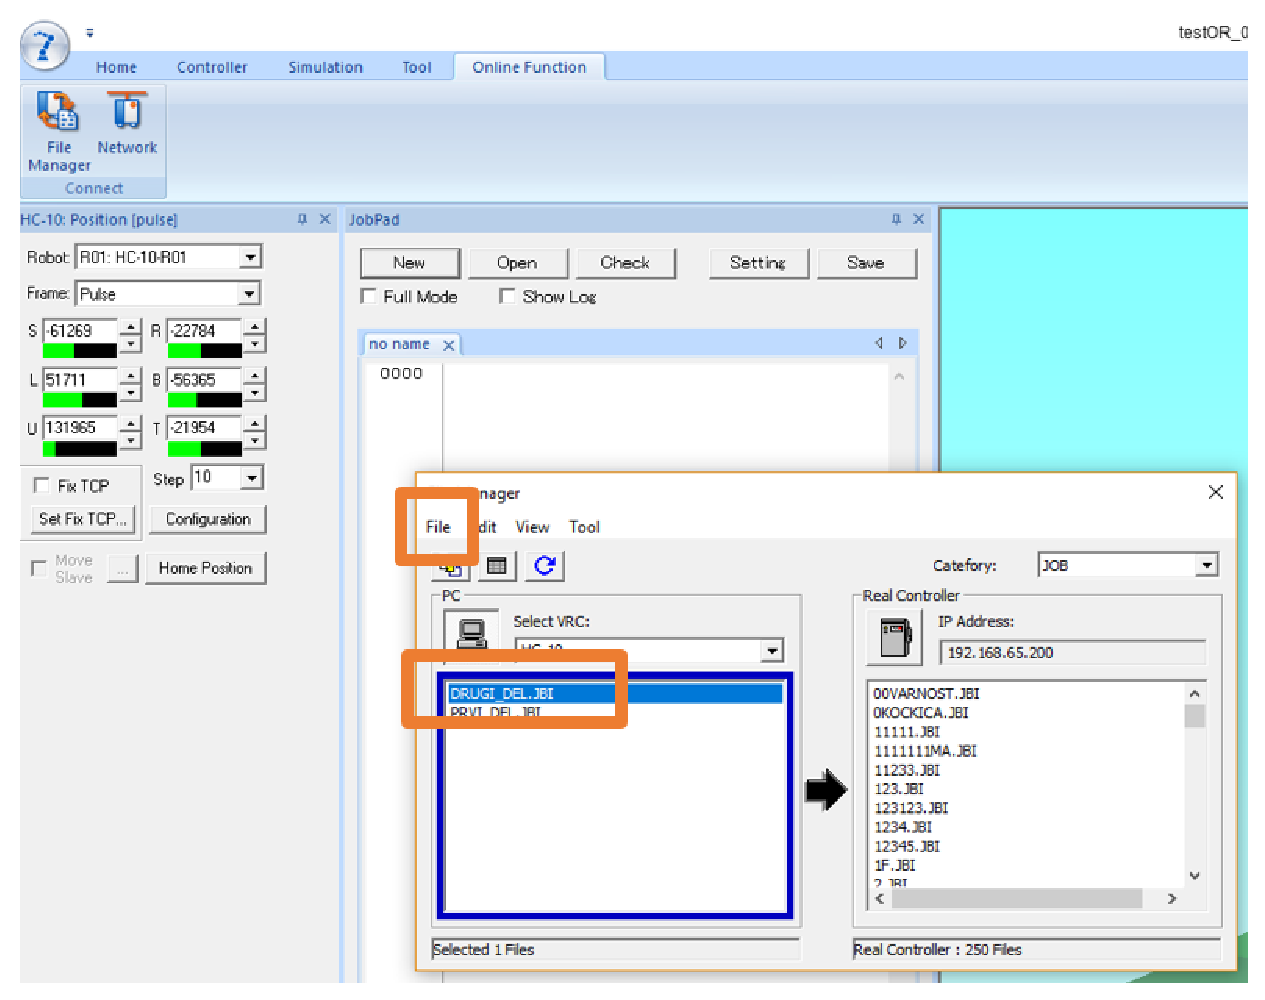
\includegraphics[width=0.7\textwidth]{VRC_15.eps}
	\caption{Prenos programa iz MotoSim okolja na dejanski krmilnik robota.}
	\label{fig:VRC_15}
\end{figure}

\subsection{Izvedba naloge} \label{realni2}


Najprej z robotom definirajte pravokotnik s šestimi točkami kot je prikazano na sliki \ref{fig:hc10_move}. Za shranjevanje točk uporabite ukaz za linearni premik \verb"MOVL V=900.0".

Testirajte napisani program, da preverite, če se robot ustrezno premika po postavljenem pravokotniku. Najprej testirajte premikanje od točke do točke (gumb \textbf{FWD}), nato pa še v avtomatskem načinu (postavite se na začetek programa, ključ na ročni učni enoti obrnite na srednji pozicijo, prižgite motorje - tipka \textbf{SERVO ON READY} in poženite program z zeleno tipko na vrhu učne enote).

\begin{figure}[!hbt]
	\centering
	\includegraphics[width=\textwidth]{hc10_move.eps}
	\caption{Testni pravokotnik, sestavljen iz šestih točk (P1 -- P6). Zelena črta označuje območje, kjer je vklopljena funkcija varnostnega odmika. }
	\label{fig:hc10_move}
\end{figure}

Ko ste zadovoljni z gibanjem robota, program nadgradite tako, da je v zelenem območju (glej sliko \ref{fig:hc10_move}) aktivirana funkcija varnostnega odmika. S klicem \verb"EI LEVEL= 1" prekinitveno funkcijo vklopite, s klicem \verb"DI LEVEL= 1" pa jo izklopite. Do \verb"EI" in \verb"DI" dostopate preko tipke \textbf{INFORM LIST} in menija \textbf{Control}. Izbiro potrdite s tipko insert \textbf{ENTER}. Nato se v programu s smernimi tipkami postavite desno na \verb"EI" (oziroma \verb"DI") in izberete \textbf{Select}. Pod izbiro \textbf{INT LEVEL} spremenite \textbf{UNUSED} v \textbf{LEVEL=} ter nastavite na \textbf{1}. Nastavitev potrdite z dvema \textbf{ENTER}.

Pred zagonom nastavite še ciklično izvajanje programa (pomeni, da se izvede en cikel). V meniju \textbf{JOB} izberete podmeni \textbf{CYCLE}. V podmeniju nastavite \textbf{WORK SELECT} na \textbf{CYCLE}, kar potrdite s tipko \textbf{ENTER}.

\vspace{5mm}

\begin{mdframed}[backgroundcolor=red!20, shadow=true,roundcorner=8pt]
	\begin{itemize}
		\item \textbf{Pokličite asistenta in delovanje funkcije varnostnega odmika testirajte SKUPAJ z asistentom!}		
	\end{itemize}
\end{mdframed}


\section{III. del: Nadzor hitrosti in oddaljenosti}

Ta način zagotavljanja varnosti prilagaja hitrost gibanja robota glede na oddaljenost operaterja od robota. Deluje po principu bližje kot je operater, počasneje se robot giblje. S tem se zagotovi efektivnost robota (deluje s polno hitrostjo, ko ni nevarnosti kontakta s človekom) ter varnost ljudi, saj se ob prisotnosti oseb robot giblje počasneje, kar pomeni, da je ob potencialnem trku manjši prenos energije. Pri implementaciji nadzora hitrosti in varnostne razdalje je potrebno implementirali dodatne zunanje senzorje, kot so laserski skenerji, pohodne plošče ali svetlobne zavese. Na sliki \ref{fig:hc10_sdm} je prikazan primer implementacije takega varnostnega protokola.

\begin{figure}[!hbt]
	\centering
	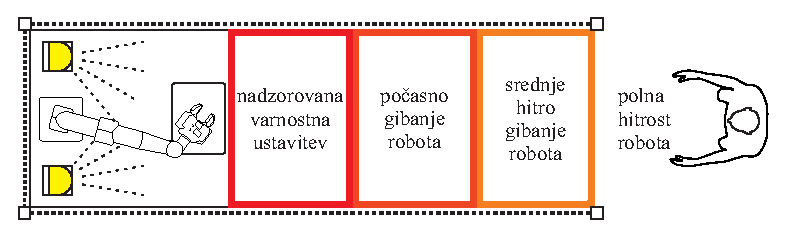
\includegraphics[width=\textwidth]{hc10_sdm.eps}
	\caption{Primer različnih področij hitrosti robota; bolj kot je področje oddaljeno, hitreje se robot lahko premika.}
	\label{fig:hc10_sdm}
\end{figure}

\subsection*{Izvedba naloge}

Pri tej nalogi boste definirali eno varnostno območje. če se bo v tem območju nahajala oseba, boste omejili gibanje robota na hitrost 50~mm/s, drugače pa se bo robot gibal s hitrostjo 250~mm/s. Za spremljanje prisotnosti človeka v varnostnem območju boste uporabili dodatni laserski skener proizvajalca SICK.

\subsubsection*{Nastavitev laserskega skenerja SICK TIM310}

V prvem delu naloge boste ustrezno sprogramili laserski skener. Pred programiranjem naprave se prepričajte, da je naprava fizično priklopljena na napajanje -- na senzorju sveti zelena LED.

Senzor priključite na računalnik preko USB kabla. Na računalniku se samodejno zažene programska oprema SOPAS, ki samodejno prepozna priključeno napravo. Za urejanje nastavitev je potrebno klikniti na ikono prepoznane naprave, ki je prikazana na sliki \ref{fig:hc10_sick1}.

\begin{figure}[!hbt]
	\centering
	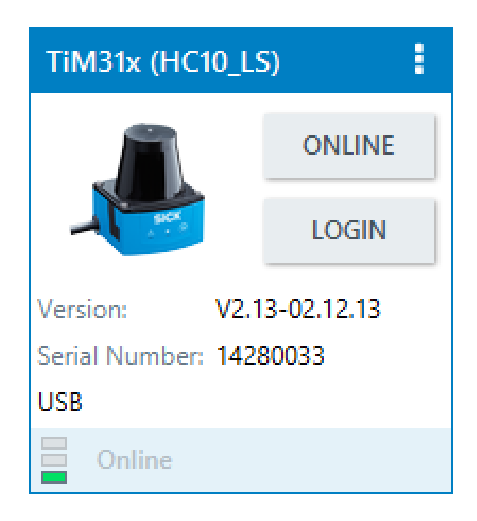
\includegraphics[width=0.3\textwidth]{hc10_sick1.eps}
	\caption{Prikaz prepoznane naprave znotraj programskega okolja SOPAS}
	\label{fig:hc10_sick1}
\end{figure}

Odpre se vam okno za urejanje nastavitev naprave, kjer se na levi strani nahaja drevesna struktura. Deli se na tri osnovne mape: \emph{Parameter}, \emph{Monitor} in \emph{Service}. Za prilagajanje delovanja senzorja je potrebno urediti nastavitve znotraj mape \textbf{Parameter} (slika \ref{fig:hc10_sick2}).

\begin{figure}[!hbt]
	\centering
	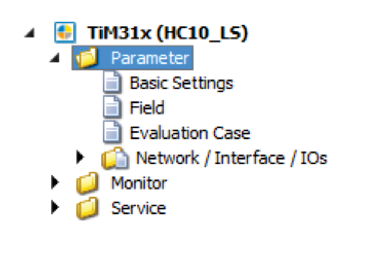
\includegraphics[width=0.3\textwidth]{hc10_sick2.eps}
	\caption{Drevesna struktura nastavitev laserskega skenerja}
	\label{fig:hc10_sick2}
\end{figure}

Najprej uredite ustrezno obliko območja znotraj katerega želimo, da senzor prepozna morebitno prisotnost. Območje naj bo po obliki in dimenziji približno enako polju, kot je prikazano na sliki \ref{fig:hc10_sick3}. Območje uredite z orodji, ki jih lahko opazimo na levi strani slike \ref{fig:hc10_sick3} (označena s številkami 1 -- 4).
\begin{itemize}
	\item Skupina orodij 1 je namenjena urejanju točk, na katerih temelji oblika polja. Prvo orodje je namenjeno dodajanju točk, drugo orodje omogoča urejanje že obstoječih točk, tretje orodje pa je namenjeno brisanju točk.
	\item Skupina orodij 2 je namenjena avtomatskemu izločanju objektov znotraj vidnega polja naprave.
	\item Skupina orodij 3 predstavlja izris prepoznanih objektov znotraj polja.
	\item Skupina orodij 4 predstavlja način prikaza polja naprave.
\end{itemize}

\begin{figure}[!hbt]
	\centering
	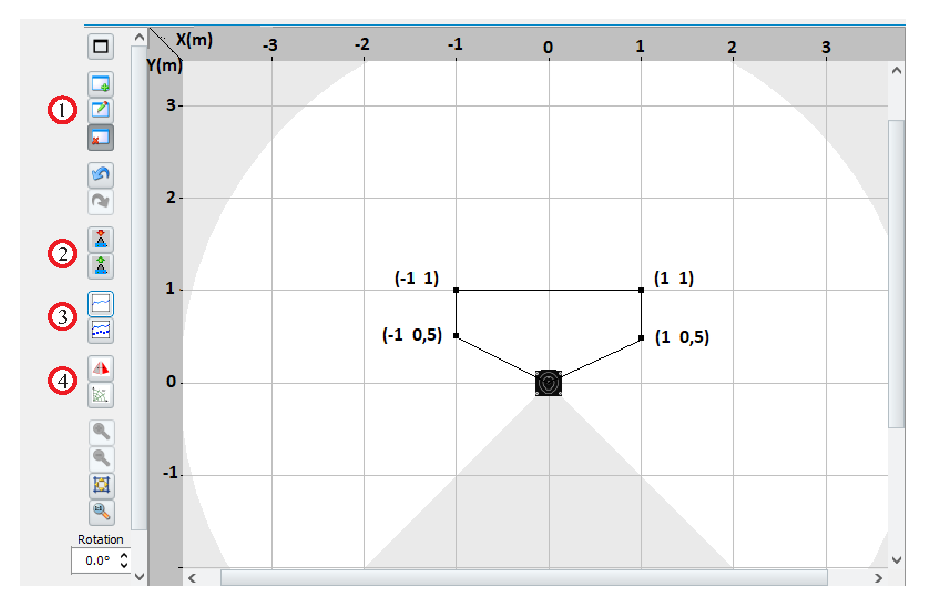
\includegraphics[width=0.9\textwidth]{hc10_sick3.eps}
	\caption{Okno za nastavljanje potrebne oblike varnostnega območja}
	\label{fig:hc10_sick3}
\end{figure}

Znotraj narisanega polja se definirajo tri varnostna območja, znotraj vsakega območja pa se spremlja morebitno prisotnost objektov. Vsako območje pro\v zi ustrezen digitalni izhod senzorja, ki je vezan naprej na FSU robotskega krmilnika. Pri vaji boste spremljali samo prisotnost osebe v srednjem območju.

Ko boste definirali ustrezno območje, definirajte tudi parametre znotraj zavihka \textbf{Evaluation Case}:
\begin{itemize}
	\item Duration time output - \v zelimo čim manjšo zakasnitev med tem, ko objekt ni več prisoten in ponovnim zagonom robota;
	\item Response time - \v zelimo, da se robot v čim krajšem času ustavi;
	\item Blanking size - \v zelimo, da senzor ne prepozna objektov manjših od 50 mm.
\end{itemize}

Z eksperimentalnim poiskušanjem poiščite ustrezne nastavitve senzorja.

Ko so vsi parametri ustrezno urejeni, zaprete okno za urejanje nastavitev naprave. Prikaže se nam opozorilo, če želimo spremembe shraniti na napravo. S tem, ko prenos potrdite, ste zaključili z nastavljanjem senzorja za prepoznavo prisotnosti. Iz senzorja izklopite USB kabel.

\subsection{Nastavitev virtualnega robotskega krmilnika} \label{sim3}

V drugem delu boste ustrezno omejili hitrosti robota glede na informacijo iz laserskega skenerja. Omejitve hitrosti se nastavljajo v meniju Safety Function/Safety Function File/Speed Limit (glej sliko \ref{fig:VRC_16}).  V tem zavihku lahko ustvarimo in nastavimo več datotek, ki omejujejo hitrost robota. Za to vajo boste ustvarili dve različni omejitvi hitrosti robota (dve datoteki): delovno hitrost ter hitrost pri interakciji (datoteka 1 in 2).


\begin{figure}[hbt]
	\centering
	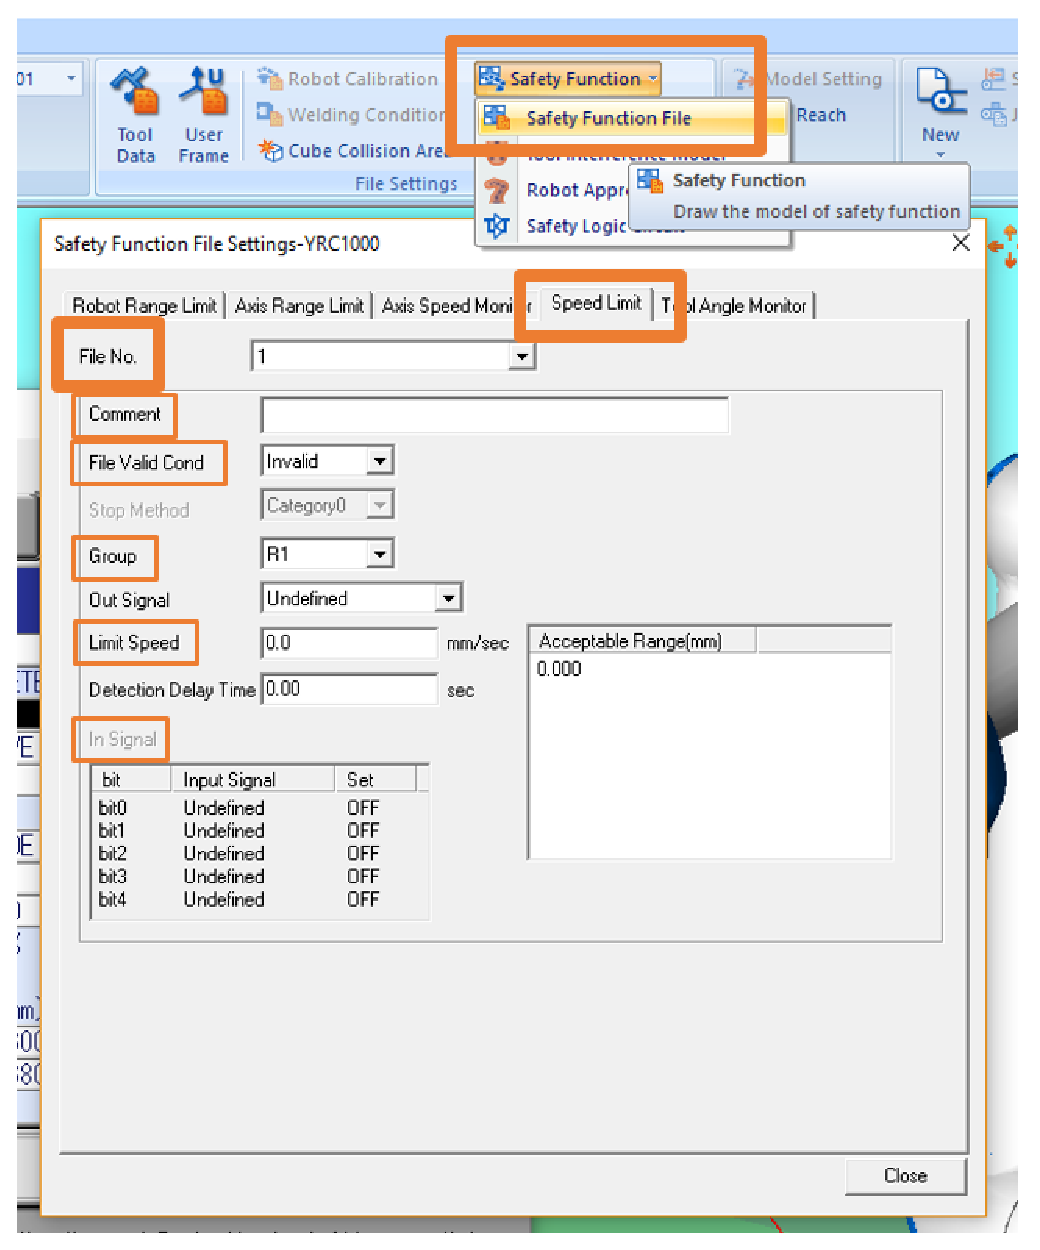
\includegraphics[width=0.7\textwidth]{VRC_16.eps}
	\caption{Okno za omejitev hitrosti}
	\label{fig:VRC_16}
\end{figure}

Delovno hitrost nastavite tako, da odprete prvo datoteko. V tem oknu morate ustrezno izpolniti polja \textbf{Comment}, \textbf{File Valid Cond}, \textbf{Group} ter \textbf{Limit Speed}.

V prvo datoteko boste nastavili vrednosti za delovno hitrost.

\begin{itemize}
	\item V polje \textbf{Comment} vpišete komentar datoteke (npr. delovna hitrost).
	\item V polju \textbf{File Valid Cond} nastavite, kdaj velja ta omejitev hitrosti. Lahko izbirate med \textbf{Valid}, ko omejitev velja vedno, \textbf{Signal}, ko želite, da je omejitev hitrosti aktivna ob določenem pogoju (signalu), in {\textbf{Invalid}}, ko ne želite, da je omejitev aktivna. Pri tej hitrosti želite, da je omejitev vedno aktivna.
	\item V polju \textbf{Group} nastavite, za katerega robota velja omejitev hitrosti. V vašem primeru imate samo enega robota, zato nastavite na \textbf{R1}.
	\item V polju \textbf{Limit Speed} definirate dejansko omejitev hitrosti. Za delovno hitrost nastavite omejitev na 250~mm/s.
\end{itemize}

V drugo datoteko boste nastavili vrednosti za hitrost pri interakciji.

\begin{itemize}
	\item V polje \textbf{Comment} vpišete komentar datoteke (npr. hitrost pri interakciji).
	\item V polju \textbf{{File Valid Cond}} nastavite, kdaj velja ta omejitev hitrosti. Ta  omejitev naj bo aktivna takrat, ko laserski skener zazna osebo v svojem varnostnem območju, zato nastavite parameter na \textbf{Signal}. Ob tem se vam pojavi dodatna možnost \textbf{In Signal}, kjer lahko definirate več pogojev oziroma signalov s poljubno logiko (\textbf{bit0} -- \textbf{bit4}). V vašem primeru gledate samo signal laserskega skenerja, ki je v robotksem krmilniku vezan na digitalni vhod  \textbf{FSBIN02( \#1)} z negativno logiko. Ta signal nastavite v polju \textbf{bit0}, kot je prikazano na sliki \ref{fig:VRC_17}. S parametrom \textbf{Set} nastavite negativno logiko (parameter nastavite na \emph{OFF}). Negativna logika pomeni to, da laserski skener postavi digitalni izhod na nizek nivo, ko zazna prisotnost osebe v varnostnem območju, v nasprotnem primeru pa je digitalni izhod postavljen na visok nivo.
	\item V polju \textbf{Group} nastavite na \textbf{R1}.
	\item V polju \textbf{Limit Speed} definirate dejansko omejitev hitrosti. Za hitrost ob potencialni interakciji nastavite omejitev na 50~mm/s.
\end{itemize}

\begin{figure}[hbt]
	\centering
	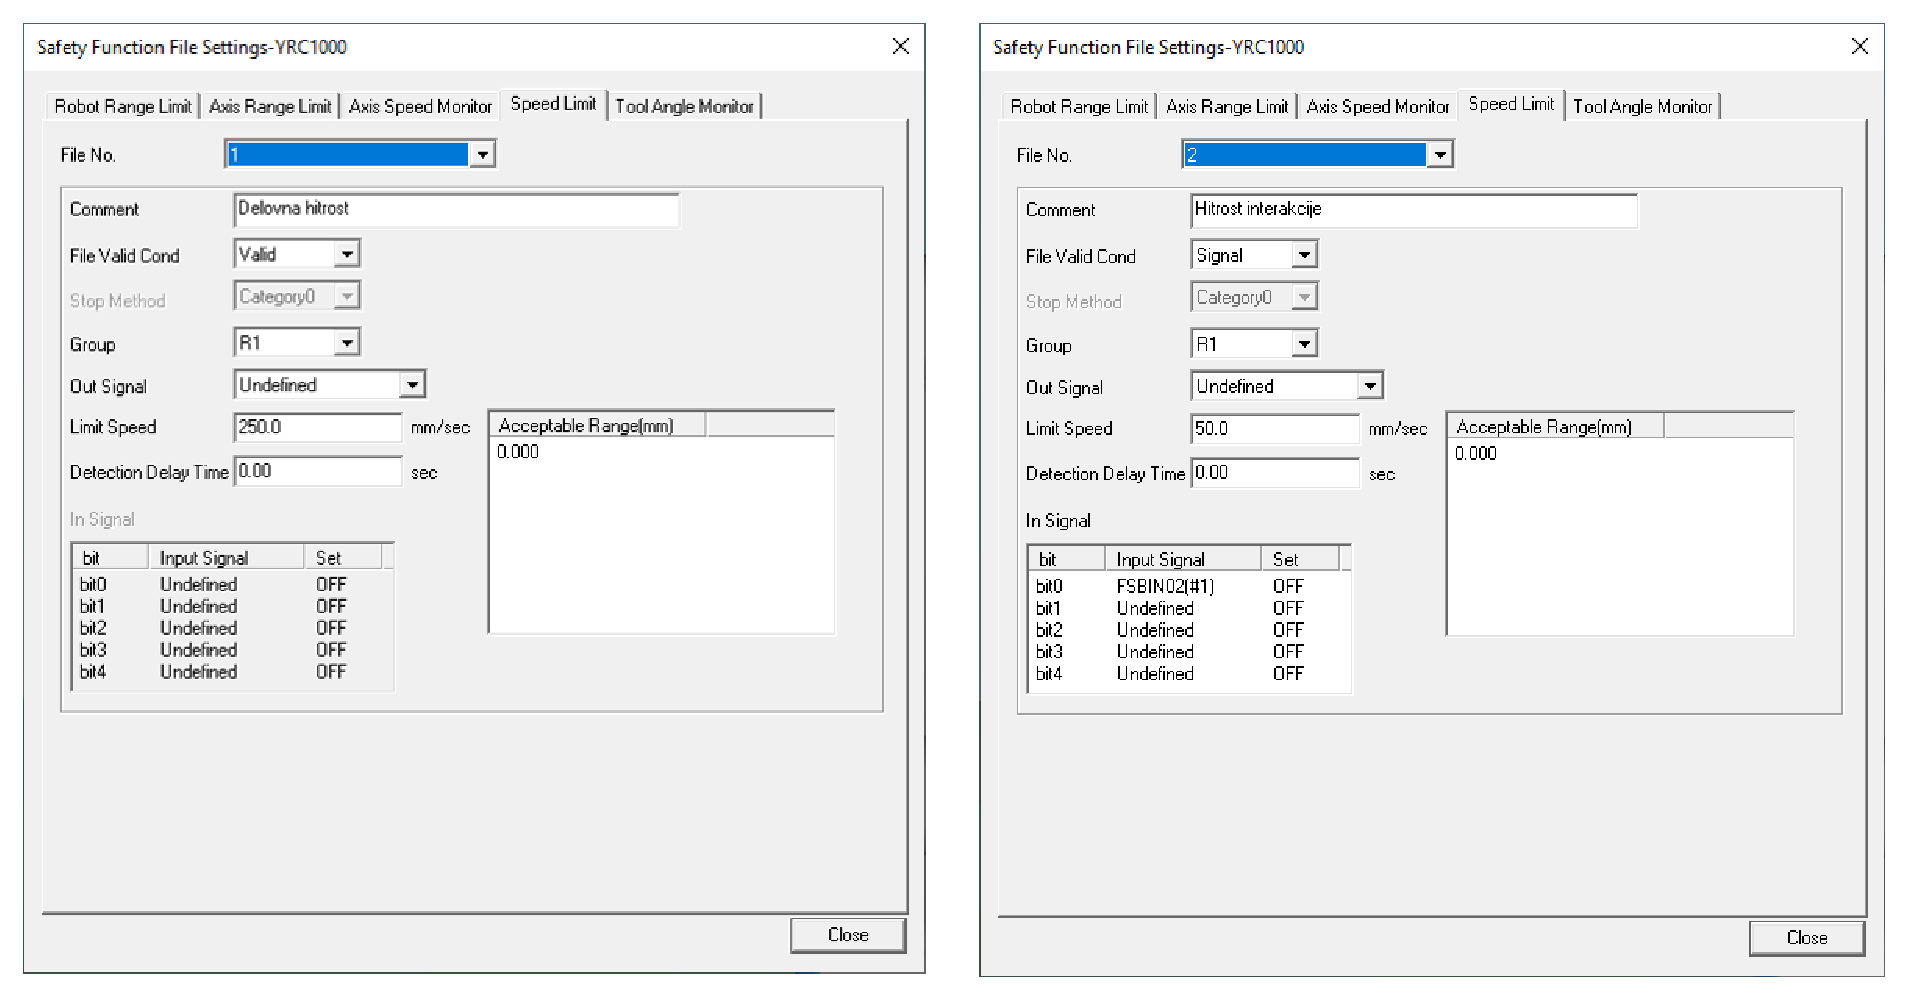
\includegraphics[width=0.7\textwidth]{VRC_17.eps}
	\caption{Okno za omejitev hitrosti za delvno hitrost in hitrost pri interakciji, ki je vezana na izhod senzorja.}
	\label{fig:VRC_17}
\end{figure}

Za test omejitev hitrosti na robotu je potrebno prenesti datoteko SPDLMT.DAT z uporabo USB ključka na dejanski krmilnik robota.

\subsection{Testiranje omejevanja hitrosti} \label{test3del}

\begin{mdframed}[backgroundcolor=red!20, shadow=true,roundcorner=8pt]
	\begin{itemize}
		\item \textbf{Pri delu od doma pokličite asistenta in delovanje funkcije omejevanja hitrosti testirate SKUPAJ z asistentom!}		
	\end{itemize}
\end{mdframed}

Za testiranje funkcionalnosti omejevanja hitrosti izberite vaš program, ki ste ga napisali v II. delu. Poženite ga v \textbf{RUN} načinu: postavite se na začetek programa, ključ na učni enoti postavite na srednjo pozicijo, prižgite motorje s \textbf{SERVO ON READY} in pritisnete zeleni gumb na vrhu učne enote.

Za testiranje se odmaknite iz vidnega polja senzorja. Robot se mora premikati s hitrostjo 250~mm/s. Ko nekdo vstopi v varnostno območje senzorja, se mora hitrost robota opazno zmanjšati na 50~mm/s.

Na podoben način bi lahko definirali še omejitve hitrosti za ostali dve območji. Pri tem bi območje najbližje robotu (najbolj nevarno zaradi največje možnosti trka) zahtevalo vklop varnostno nadzorovane ustavitve.



